\subsection{Validation Metric Details}
\label{sec:metric_details}

This appendix documents the precise form of the seven per-path metrics referenced in Section~\ref{sec:metrics}.
For each model, 1{,}000 independent paths of length $T$ are simulated (200 paths for the cross-asset extension) and each metric is computed per path before aggregation.

\paragraph{Kolmogorov--Smirnov (KS) pass rate.}
The two-sample KS statistic \cite{kolmogorov1933, smirnov1948} measures the maximum vertical distance between two empirical CDFs,
\begin{equation}
    D_{n,m} = \sup_x |F_n(x) - G_m(x)|.
    \label{eq:ks}
\end{equation}
The KS pass rate is the fraction of paths for which the test fails to reject distributional equivalence against the reference data at $\alpha = 0.05$.

\paragraph{Anderson--Darling (AD) pass rate.}
The AD test is the integrated squared CDF deviation with a quadratic tail weighting, making it more sensitive than KS to tail discrepancies.
The AD pass rate is the fraction of paths for which the two-sample AD test fails to reject at $\alpha = 0.05$.

\paragraph{Excess kurtosis.}
Mean simulated excess kurtosis across paths, compared to the observed value.
Given Gaussian emissions, the CHMM is expected to underestimate kurtosis relative to the heavy-tailed empirical distribution, and the shortfall is one of the reported diagnostics.

\paragraph{ACF-MAE.}
Mean absolute error between observed and mean-simulated autocorrelation functions of $|G_t|$ over $L = 252$ lags,
\begin{equation}
    \text{ACF-MAE} = \frac{1}{L}\sum_{\tau=1}^{L} \left| \hat\rho^{\text{obs}}_{|G|}(\tau) - \bar{\hat\rho}^{\,\text{sim}}_{|G|}(\tau) \right|.
    \label{eq:acf_mae_supp}
\end{equation}
This is the direct diagnostic for the Ryd\'{e}n et al.\ limitation.

\paragraph{Wasserstein-1 distance.}
The mean absolute difference of sorted empirical quantiles, equivalent to the $L^1$ distance between the empirical CDFs \cite{glasserman2003monte},
\begin{equation}
    W_1(F, G) = \int_0^1 |F^{-1}(u) - G^{-1}(u)|\, du.
    \label{eq:wasserstein}
\end{equation}

\paragraph{Hellinger distance.}
A histogram-based overlap distance in $[0, 1]$,
\begin{equation}
    H(P, Q) = \frac{1}{\sqrt{2}}\sqrt{\sum_{i=1}^{B}\left(\sqrt{p_i} - \sqrt{q_i}\right)^2},
    \label{eq:hellinger}
\end{equation}
with $B$ equal-width bins spanning the joint support and $p_i, q_i$ the observed and simulated bin probabilities.

\paragraph{Quantile coverage.}
The fraction of 99 equally-spaced observed quantiles (1st through 99th percentile) falling inside the 5th--95th percentile envelope of the corresponding simulated quantile across 1{,}000 paths.
A coverage of 100\% indicates that the simulation envelope fully brackets the observed distribution at every percentile.

\paragraph{Cross-asset metrics.}
For the cross-asset extension we additionally track the mean Frobenius norm $\|\hat\Sigma_{\text{sim}}^{(p)} - \hat\Sigma_{\text{obs}}\|_F$ and the off-diagonal Pearson correlation MAE between simulated and observed return matrices, averaged over paths.

\subsection{Forward-Backward Recursions and M-Step Updates}
\label{sec:baum_welch_supp}

For reference, the in-text Baum-Welch description of Section~\ref{sec:chmm_def} is underpinned by the standard log-space recursions \cite{rabiner1986introduction, bilmes1998gentle}.
Define the forward variable $\alpha_t(k) = \Prob(O_{1:t}, S_t = k \mid \mathcal{M})$ and the backward variable $\beta_t(k) = \Prob(O_{t+1:T} \mid S_t = k, \mathcal{M})$.
The log-space recursions are
\begin{align}
    \log \alpha_1(k) &= \log \pi_k + \log b_k(O_1), \label{eq:forward_init} \\
    \log \alpha_t(j) &= \underset{i}{\text{logsumexp}}\!\left(\log \alpha_{t-1}(i) + \log T_{ij}\right) + \log b_j(O_t), \quad t = 2, \ldots, T, \label{eq:forward} \\[4pt]
    \log \beta_T(k) &= 0, \label{eq:backward_init} \\
    \log \beta_t(i) &= \underset{j}{\text{logsumexp}}\!\left(\log T_{ij} + \log b_j(O_{t+1}) + \log \beta_{t+1}(j)\right), \quad t = T{-}1, \ldots, 1, \label{eq:backward}
\end{align}
where $\text{logsumexp}_i(x_i) = x_{\max} + \log \sum_i \exp(x_i - x_{\max})$.
The posterior state-occupancy $\gamma_t(k)$ and pair-occupancy $\xi_t(i, j)$ quantities are
\begin{equation}
    \gamma_t(k) = \frac{\alpha_t(k) \beta_t(k)}{\sum_j \alpha_t(j) \beta_t(j)}, \qquad
    \xi_t(i, j) = \frac{\alpha_t(i)\, T_{ij}\, b_j(O_{t+1})\, \beta_{t+1}(j)}{\sum_{m,n} \alpha_t(m)\, T_{mn}\, b_n(O_{t+1})\, \beta_{t+1}(n)},
    \label{eq:gamma_xi}
\end{equation}
and the closed-form M-step updates are
\begin{equation}
    \pi_k^{\text{new}} = \gamma_1(k),\quad
    \mu_k^{\text{new}} = \frac{\sum_t \gamma_t(k)\, O_t}{\sum_t \gamma_t(k)},\quad
    \left(\sigma_k^{\text{new}}\right)^2 = \frac{\sum_t \gamma_t(k)(O_t - \mu_k^{\text{new}})^2}{\sum_t \gamma_t(k)},\quad
    T_{ij}^{\text{new}} = \frac{\sum_{t=1}^{T-1} \xi_t(i, j)}{\sum_{t=1}^{T-1} \gamma_t(i)}.
    \label{eq:mstep}
\end{equation}
The convergence criterion is $|\mathcal{L}^{(n)} - \mathcal{L}^{(n-1)}| < 10^{-4}$ with $\mathcal{L}^{(n)} = \text{logsumexp}_k \log \alpha_T^{(n)}(k)$, and simulation draws $S_1 \sim \text{Categorical}(\boldsymbol{\pi})$ and then iterates $G_t \sim \mathcal{N}(\mu_{S_t}, \sigma_{S_t}^2)$, $S_{t+1} \sim \text{Categorical}(\mathbf{T}_{S_t, \cdot})$ with no jump process.

\paragraph{CHMM-t M-step (per-state ECM, closed form given $u_{t,k}$).}
For Student-t emissions $b_k(x) = t_{\nu_k}(x; \mu_k, \sigma_k)$ the ECM formulation of \citet{peel2000robust, liu1995ml} treats the latent precision as an augmented E-step quantity,
\begin{equation}
    u_{t,k} = \frac{\nu_k + 1}{\nu_k + ((O_t - \mu_k)/\sigma_k)^2},
    \label{eq:tprecision_supp}
\end{equation}
so that conditional on $\nu_k$ the location and scale admit closed-form weighted updates,
\begin{equation}
    \mu_k^{\text{new}} = \frac{\sum_t \gamma_t(k)\, u_{t,k}\, O_t}{\sum_t \gamma_t(k)\, u_{t,k}},\quad
    \left(\sigma_k^{\text{new}}\right)^2 = \frac{\sum_t \gamma_t(k)\, u_{t,k}\, (O_t - \mu_k^{\text{new}})^2}{\sum_t \gamma_t(k)}.
    \label{eq:tupdate_supp}
\end{equation}
The degrees-of-freedom parameter $\nu_k$ is then refined by a one-dimensional golden-section search on the per-state $Q$-function $Q_k(\nu) = \sum_t \gamma_t(k)\, \log t_\nu(O_t; \mu_k, \sigma_k)$ over the bracket $(\nu_{\min}, \nu_{\max}) = (2.1, 50)$.
This two-block ECM preserves the monotonicity of the standard EM guarantee.

\paragraph{CHMM-L M-step (closed-form weighted Laplace MLE).}
For Laplace emissions $b_k(x) = \tfrac{1}{2 b_k} \exp(-|x - \mu_k|/b_k)$ the weighted-MLE estimators are available in closed form:
\begin{equation}
    \mu_k^{\text{new}} = \text{WeightedMedian}\!\left(O_{1:T};\, \gamma_{1:T}(k)\right),\qquad
    b_k^{\text{new}} = \frac{\sum_t \gamma_t(k)\, |O_t - \mu_k^{\text{new}}|}{\sum_t \gamma_t(k)}.
    \label{eq:lupdate_supp}
\end{equation}
The weighted median is computed by cumulative-weight bracketing with linear interpolation between adjacent order statistics at the half-total weight crossing.
The Laplace M-step carries no shape parameter, so CHMM-L is strictly cheaper per iteration than CHMM-t (which requires the per-state $Q_k$ search).

\subsection{Full State-Resolution Sensitivity Table}
\label{sec:sensitivity_table}

Table~\ref{tab:sensitivity} reports the full sweep summarized by Figure~\ref{fig:k_sweep_summary} in the main text.
Observed excess kurtosis is 7.71 IS and 6.24 OoS at all $K$.

\begin{table}[H]
\centering
\caption{State resolution sensitivity for SPY CHMM (1{,}000 paths, $\alpha = 0.05$). Every metric is computed on the identical simulation pipeline used for Table~\ref{tab:model_comparison} in the main text. Coverage was 100\% at every $K$ in both IS and OoS windows.}
\label{tab:sensitivity}
\small
\begin{tabular}{c cc cc cc c c c c}
\toprule
& \multicolumn{2}{c}{KS (\%)} & \multicolumn{2}{c}{AD (\%)} & \multicolumn{2}{c}{Kurtosis} & & & & \\
\cmidrule(lr){2-3} \cmidrule(lr){4-5} \cmidrule(lr){6-7}
$K$ & IS & OoS & IS & OoS & Obs & Sim & ACF-MAE & $W_1$ & $H$ & Cov (\%) \\
\midrule
3  & 88.7 & 92.8 & 79.2 & 84.9 & 7.71 & 3.91 & 0.0453 & 0.119 & 0.0793 & 100.0 \\
6  & 90.3 & 93.8 & 83.6 & 87.0 & 7.71 & 5.13 & 0.0488 & 0.110 & 0.0786 & 100.0 \\
9  & 91.7 & 92.4 & 83.2 & 85.3 & 7.71 & 3.70 & 0.0473 & 0.115 & 0.0779 & 100.0 \\
12 & 95.3 & 91.9 & 87.2 & 85.0 & 7.71 & 4.19 & 0.0483 & 0.108 & 0.0767 & 100.0 \\
15 & 93.5 & 94.0 & 86.8 & 87.0 & 7.71 & 4.46 & 0.0490 & 0.105 & 0.0765 & 100.0 \\
\textbf{18} & 95.2 & 94.0 & 88.3 & 88.7 & 7.71 & 5.03 & 0.0505 & 0.101 & 0.0771 & 100.0 \\
21 & \textbf{96.5} & \textbf{94.9} & \textbf{89.1} & 87.0 & 7.71 & 4.71 & 0.0503 & 0.103 & 0.0777 & 100.0 \\
\bottomrule
\end{tabular}
\end{table}

\subsection{Multi-Emission State-Resolution Sensitivity}
\label{sec:multi_emission_sensitivity}

Table~\ref{tab:sensitivity_multi} extends Table~\ref{tab:sensitivity} across the three emission families, confirming that the qualitative operating point $K = 18$ is stable when the Gaussian component is replaced with Student-t or Laplace emissions.
For CHMM-t the per-state degrees of freedom $\nu_k$ are refit by ECM-plus-golden-section at every $K$; for CHMM-L the weighted-median location and weighted MAD scale are closed form and impose no additional cost.
Three patterns extend from Table~\ref{tab:sensitivity} to the new families.
First, the distributional pass rates plateau in the $K \in \{12, 15, 18, 21\}$ band for all three families: CHMM-t reaches its highest IS KS at $K = 15$ (96.3\%) and its highest OoS KS at $K = 18$ (95.6\%), and CHMM-L reaches its highest IS AD at $K = 12$ (91.1\%) and its highest OoS AD at $K = 18$ (92.6\%).
Once a family enters the plateau the operating point is flat with respect to $K$, so we report the main-text results at the same $K = 18$ used for CHMM-N.
Second, the ACF-MAE remains within the narrow 0.045--0.055 band observed for the Gaussian sweep, indicating that the volatility-clustering mechanism is a property of the regime structure rather than the emission family.
Third, simulated kurtosis behaves as expected from the component families: the Gaussian sweep peaks at 5.1, the Laplace sweep lands squarely in the 5.1--6.5 range (closest to the observed 7.71), and the Student-t sweep climbs sharply above 10 across the entire sweep because the ECM search assigns small $\nu_k$ to a subset of tail states, over-correcting in-sample kurtosis but aligning OoS.

\begin{table}[H]
\centering
\caption{Multi-emission state resolution sensitivity for SPY (1{,}000 paths, $\alpha = 0.05$). CHMM-N: Gaussian; CHMM-t: Student-t with per-state $\nu_k$ refit by ECM-plus-golden-section; CHMM-L: Laplace with weighted-median location and weighted-MAD scale. Every metric is computed on the identical simulation pipeline used for Table~\ref{tab:model_comparison}. Quantile coverage is 100\% at every $(K, \text{family})$ cell in both IS and OoS windows with the single exception of CHMM-L at $K = 3$ (88.9\% IS, 100.0\% OoS). Observed excess kurtosis is 7.71 IS and 6.24 OoS.}
\label{tab:sensitivity_multi}
\small
\resizebox{\textwidth}{!}{%
\begin{tabular}{l c cc cc c c c c}
\toprule
& & \multicolumn{2}{c}{KS (\%)} & \multicolumn{2}{c}{AD (\%)} & & & & \\
\cmidrule(lr){3-4} \cmidrule(lr){5-6}
Family & $K$ & IS & OoS & IS & OoS & Kurt (IS sim) & ACF-MAE & $W_1$ IS & $H$ IS \\
\midrule
CHMM-N & 3  & 88.7 & 92.8 & 79.2 & 84.9 & 3.91 & 0.0453 & 0.119 & 0.0793 \\
       & 6  & 90.3 & 93.8 & 83.6 & 87.0 & 5.13 & 0.0488 & 0.110 & 0.0786 \\
       & 9  & 91.7 & 92.4 & 83.2 & 85.3 & 3.70 & 0.0473 & 0.115 & 0.0779 \\
       & 12 & 95.3 & 91.9 & 87.2 & 85.0 & 4.19 & 0.0483 & 0.108 & 0.0767 \\
       & 15 & 93.5 & 94.0 & 86.8 & 87.0 & 4.46 & 0.0490 & 0.105 & 0.0765 \\
       & \textbf{18} & 95.2 & 94.0 & 88.3 & 88.7 & 5.03 & 0.0505 & 0.101 & 0.0771 \\
       & 21 & \textbf{96.5} & 94.9 & \textbf{89.1} & 87.0 & 4.71 & 0.0503 & 0.103 & 0.0777 \\
\midrule
CHMM-t & 3  & 92.0 & 93.0 & 90.3 & 88.1 & 28.28 & 0.0541 & 0.097 & 0.0722 \\
       & 6  & 93.3 & 94.2 & 89.2 & 87.1 & 26.01 & 0.0529 & 0.097 & 0.0729 \\
       & 9  & 94.6 & 94.4 & 89.0 & 88.2 & 17.05 & 0.0532 & 0.096 & 0.0725 \\
       & 12 & 94.8 & 94.6 & 90.0 & 89.4 & 13.23 & 0.0532 & 0.095 & 0.0723 \\
       & 15 & \textbf{96.3} & 95.2 & 90.9 & 90.3 & 14.33 & 0.0539 & 0.093 & 0.0721 \\
       & \textbf{18} & 95.3 & \textbf{95.6} & 90.1 & 89.3 & 13.40 & 0.0535 & 0.094 & \textbf{0.0719} \\
       & 21 & 96.0 & 94.7 & \textbf{91.1} & 87.5 & 12.07 & 0.0526 & \textbf{0.093} & 0.0727 \\
\midrule
CHMM-L & 3  & 77.0 & 90.3 & 80.1 & 86.0 & 5.11 & 0.0529 & 0.110 & 0.0822 \\
       & 6  & 90.1 & 91.3 & 85.2 & 83.8 & 5.87 & 0.0504 & 0.105 & 0.0786 \\
       & 9  & 91.7 & 92.8 & 86.0 & 85.5 & 6.08 & 0.0517 & 0.103 & 0.0777 \\
       & 12 & 94.6 & 94.5 & \textbf{91.1} & 89.5 & 6.41 & 0.0533 & 0.096 & 0.0758 \\
       & 15 & \textbf{94.7} & 95.0 & 90.1 & 90.5 & 6.36 & 0.0537 & 0.097 & 0.0760 \\
       & \textbf{18} & 93.2 & 94.1 & 91.0 & \textbf{92.6} & \textbf{6.45} & 0.0541 & 0.096 & 0.0761 \\
       & 21 & 93.9 & 92.7 & 89.4 & 89.5 & 5.98 & 0.0532 & 0.097 & 0.0764 \\
\bottomrule
\end{tabular}%
}
\end{table}

\subsection{Baum-Welch Convergence}
\label{sec:convergence}

Figure~\ref{fig:convergence_all} shows the Baum-Welch convergence curves for representative state resolutions.
All models converged within the 60-iteration budget, with the log-likelihood monotonically increasing (as guaranteed by the EM algorithm).
Lower $K$ values typically converged faster (15--25 iterations), while higher $K$ values required 25--40 iterations to reach the convergence tolerance of $|\Delta\mathcal{L}| < 10^{-4}$.
The monotonic increase confirms that the quantile-based initialization provided a valid starting point from which the EM algorithm could improve without encountering degenerate solutions.

\begin{figure}[H]
\centering
\begin{subfigure}[b]{0.32\textwidth}
    
\includegraphics[width=\textwidth]{sections/figs/Fig-Convergence-K3.pdf}
    \caption{$K = 3$}
\end{subfigure}
\hfill
\begin{subfigure}[b]{0.32\textwidth}
    
\includegraphics[width=\textwidth]{sections/figs/Fig-Convergence-K12.pdf}
    \caption{$K = 12$}
\end{subfigure}
\hfill
\begin{subfigure}[b]{0.32\textwidth}
    
\includegraphics[width=\textwidth]{sections/figs/Fig-Convergence-K18.pdf}
    \caption{$K = 18$ (selected)}
\end{subfigure}
\caption{Baum-Welch convergence for selected state resolutions. Log-likelihood is monotonically increasing (EM guarantee) and plateaus well before $\texttt{max\_iter} = 60$.}
\label{fig:convergence_all}
\end{figure}

\subsection{Emission Distributions Across State Resolutions}

Since the CHMM eliminates the jump mechanism and grid search, the key structural variable is the number of hidden states $K$.
Figure~\ref{fig:emissions_all} compares the learned emission distributions for $K \in \{3, 6, 12, 18\}$, illustrating how increasing state resolution refines the decomposition of the observed return distribution.

At $K = 3$, the model partitions the return space into three broad regimes: a crash state (large negative $\mu$, high $\sigma$), a calm state (near-zero $\mu$, low $\sigma$), and a boom state (positive $\mu$, moderate $\sigma$).
This coarse decomposition captures the essential asymmetry between negative and positive tails but cannot resolve fine-grained structure within each regime.

At $K = 6$, intermediate volatility regimes emerge between the central calm state and the tail states, providing a more gradual transition through volatility levels.

At $K = 12$--$18$, the emission distributions form a dense coverage of the return space, with each state capturing a narrow band of returns.
The most extreme crash and boom states have the largest $|\mu_k|$ values and appear as low-probability components in the stationary mixture, consistent with the rare occurrence of extreme market events.

\begin{figure}[H]
\centering
\begin{subfigure}[b]{0.24\textwidth}
    
\includegraphics[width=\textwidth]{sections/figs/Fig-Emission-PDFs-K3.pdf}
    \caption{$K = 3$}
\end{subfigure}
\hfill
\begin{subfigure}[b]{0.24\textwidth}
    
\includegraphics[width=\textwidth]{sections/figs/Fig-Emission-PDFs-K6.pdf}
    \caption{$K = 6$}
\end{subfigure}
\hfill
\begin{subfigure}[b]{0.24\textwidth}
    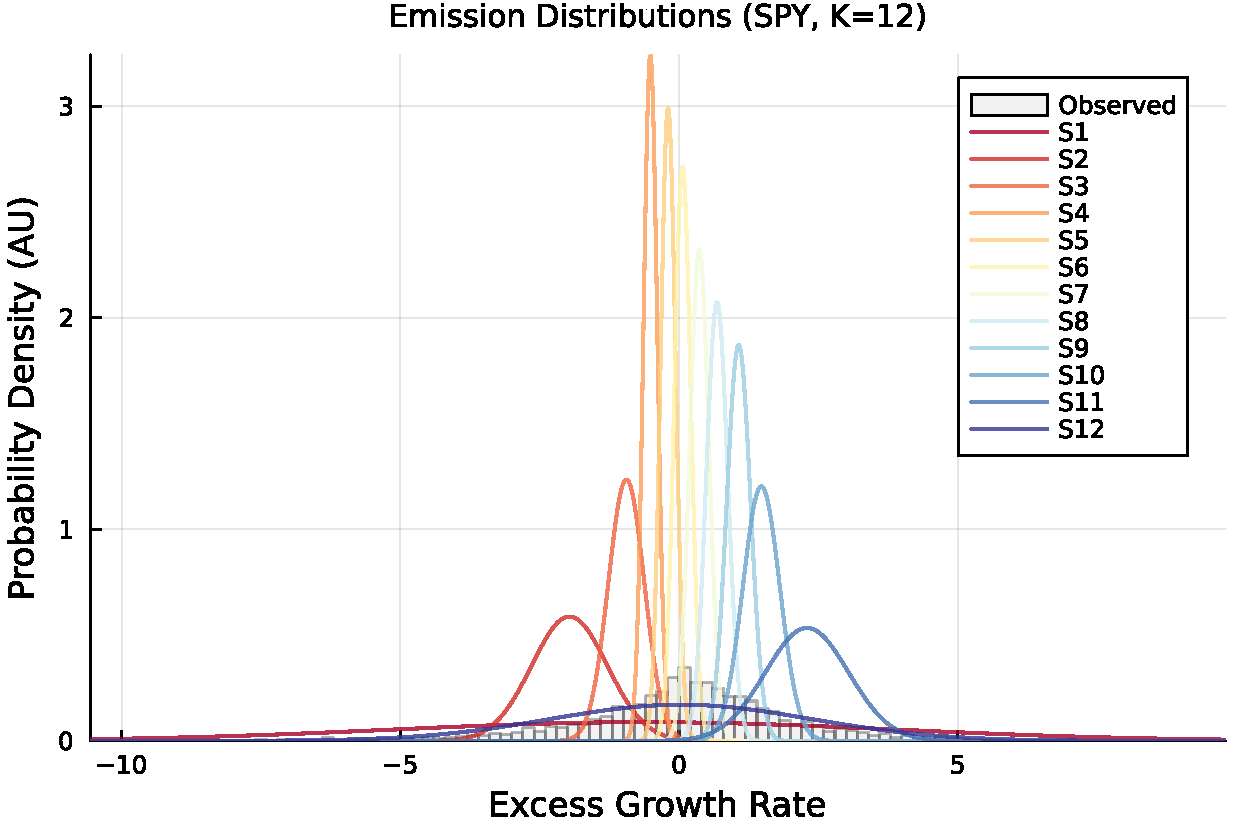
\includegraphics[width=\textwidth]{sections/figs/Fig-Emission-PDFs-K12.pdf}
    \caption{$K = 12$}
\end{subfigure}
\hfill
\begin{subfigure}[b]{0.24\textwidth}
    
\includegraphics[width=\textwidth]{sections/figs/Fig-Emission-PDFs-K18.pdf}
    \caption{$K = 18$ (selected)}
\end{subfigure}
\caption{Learned Gaussian emission distributions across state resolutions, overlaid on the observed SPY return histogram. Higher $K$ values produce finer decomposition with dedicated states capturing tail behavior.}
\label{fig:emissions_all}
\end{figure}

\subsection{Transition Matrix Structure}

Figure~\ref{fig:transition_all} shows the learned transition matrices for $K = 6$ and $K = 18$ in log$_{10}$ color scale.
Both matrices exhibit a dominant near-diagonal band, reflecting the tendency of the market to remain in its current regime.
Off-diagonal entries decay with distance from the diagonal, indicating that large regime jumps (for example, from a deep crash state directly to a boom state) are rare but nonzero.

The diagonal dominance is critical for the ACF-MAE result discussed in Section~\ref{sec:discussion}: the self-transition probabilities $T_{kk}$ for central states are typically 0.7--0.95, producing mean sojourn times of 3--20 days.
The mixture of these geometric sojourn times across states produces the sum-of-exponentials ACF profile that approximates the observed slow decay.

\begin{figure}[H]
\centering
\begin{subfigure}[b]{0.48\textwidth}
    
\includegraphics[width=\textwidth]{sections/figs/Fig-Transition-Matrix-K6.pdf}
    \caption{$K = 6$}
\end{subfigure}
\hfill
\begin{subfigure}[b]{0.48\textwidth}
    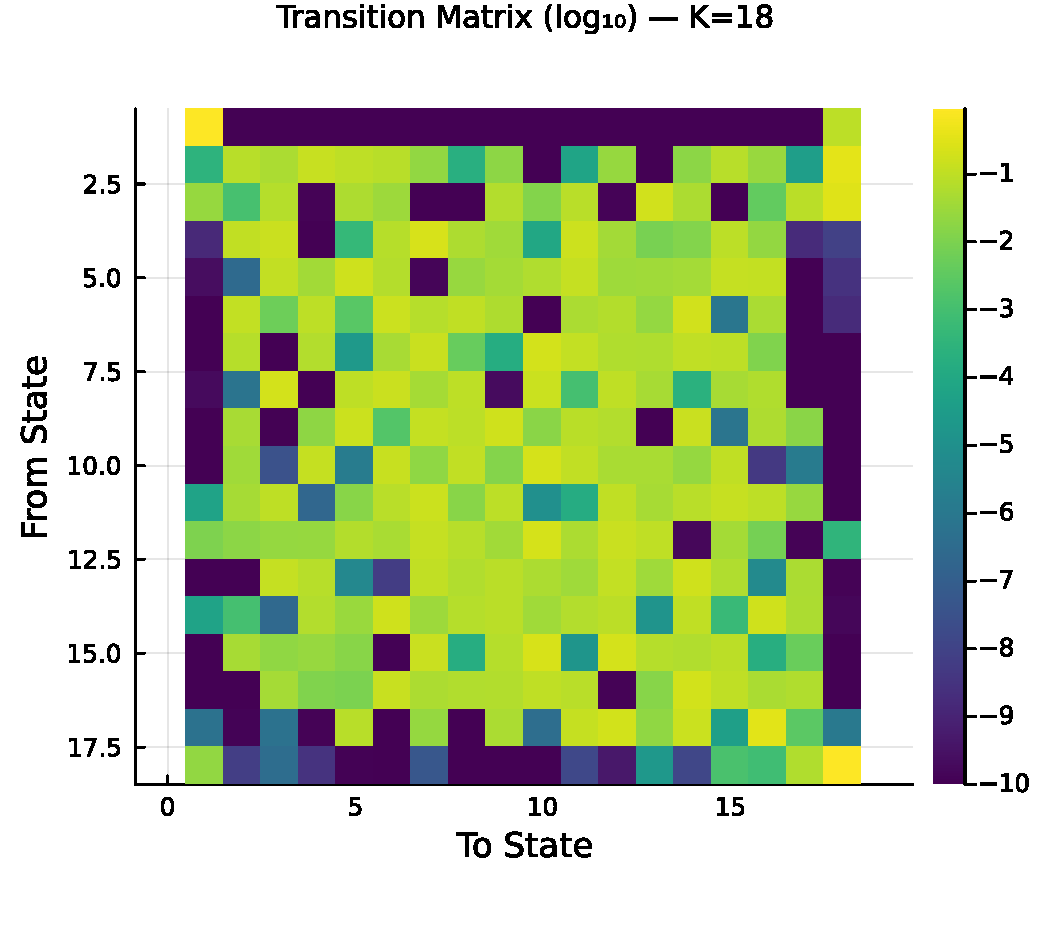
\includegraphics[width=\textwidth]{sections/figs/Fig-Transition-Matrix-K18.pdf}
    \caption{$K = 18$ (selected)}
\end{subfigure}
\caption{Learned transition matrices in log$_{10}$ color scale. The near-diagonal band reflects regime persistence; off-diagonal entries decay with distance, indicating that large regime transitions are rare.}
\label{fig:transition_all}
\end{figure}

\subsection{Stationary Distributions and Residence Times}

Figure~\ref{fig:stationary_all} shows the stationary distributions $\bar{\boldsymbol{\pi}}$ for $K = 6$ and $K = 18$.
In both cases, the central states (those with $\mu_k$ near zero and moderate $\sigma_k$) receive the highest stationary probability, consistent with the empirical concentration of returns near zero.
Tail states (crash and boom) receive low stationary probability, consistent with the rarity of extreme events.

Figure~\ref{fig:residence_all} shows the natural residence times $\tau_k = 1/(1 - T_{kk})$ per state for $K = 6$ and $K = 18$.
Under pure Markov dynamics (no jump mechanism), the expected duration in state $k$ before transitioning is $\tau_k$ steps.
Central states exhibit the longest residence times (5--20 days), while tail states have shorter residence times (1--3 days), consistent with the transient nature of extreme market events.
Notably, even without a jump mechanism, the tail states at higher $K$ maintain sufficient self-transition probability ($T_{kk} \approx 0.3$--$0.5$) to produce multi-day tail episodes.
This contrasts with the discrete model of \citet{alswaidan2026hybrid}, where tail-state residence times were too short to sustain clustering without the Poisson jump extension.

\begin{figure}[H]
\centering
\begin{subfigure}[b]{0.48\textwidth}
    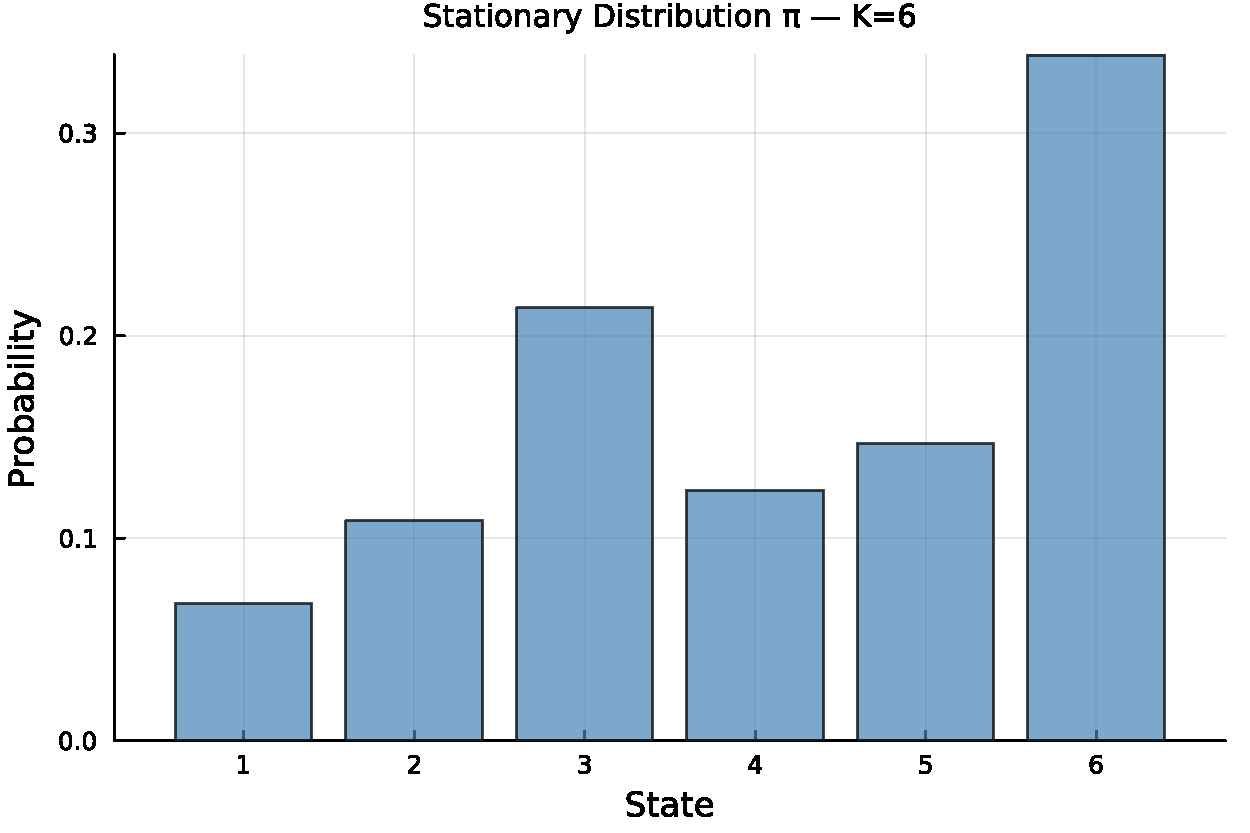
\includegraphics[width=\textwidth]{sections/figs/Fig-Stationary-Distribution-K6.pdf}
    \caption{$K = 6$}
\end{subfigure}
\hfill
\begin{subfigure}[b]{0.48\textwidth}
    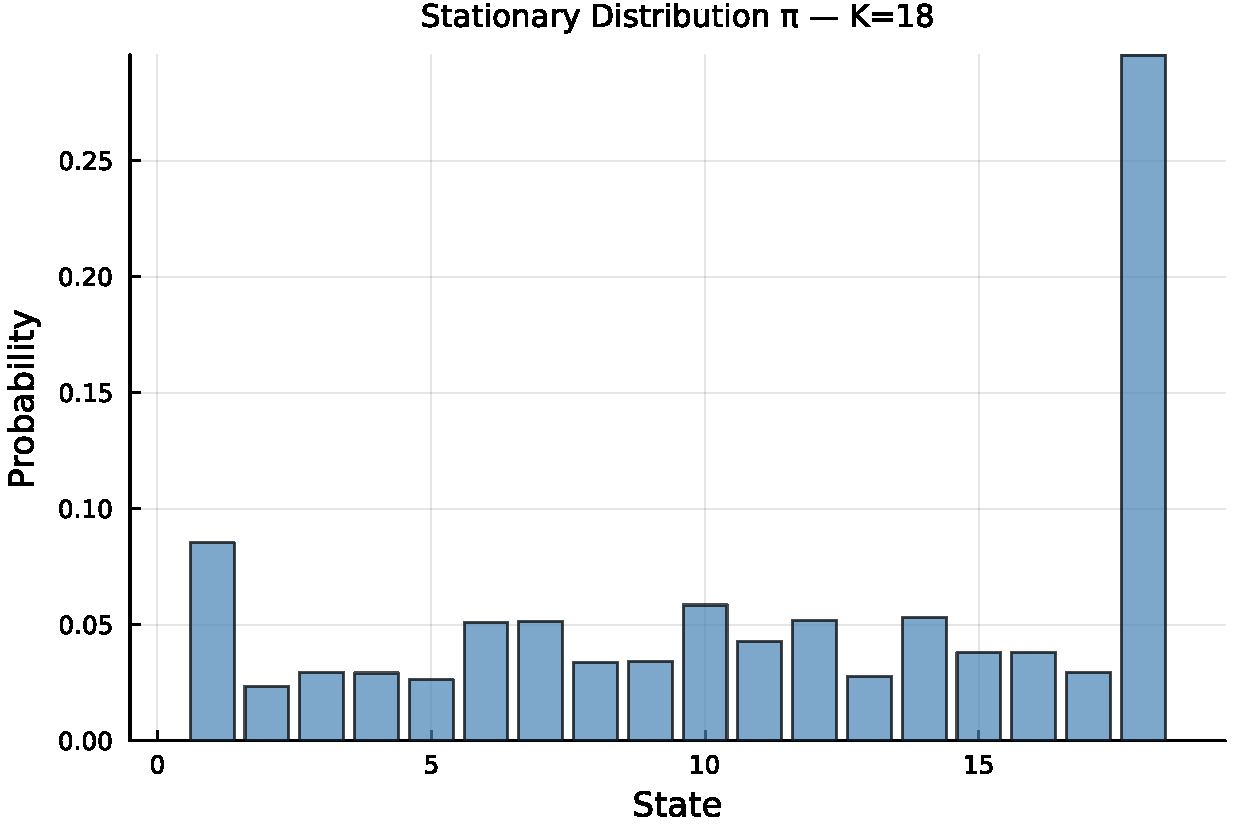
\includegraphics[width=\textwidth]{sections/figs/Fig-Stationary-Distribution-K18.pdf}
    \caption{$K = 18$}
\end{subfigure}
\caption{Stationary distributions $\bar{\boldsymbol{\pi}}$ for $K = 6$ and $K = 18$. Central states receive the highest stationary probability, consistent with the concentration of returns near zero.}
\label{fig:stationary_all}
\end{figure}

\begin{figure}[H]
\centering
\begin{subfigure}[b]{0.48\textwidth}
    
\includegraphics[width=\textwidth]{sections/figs/Fig-Residence-Times-K6.pdf}
    \caption{$K = 6$}
\end{subfigure}
\hfill
\begin{subfigure}[b]{0.48\textwidth}
    
\includegraphics[width=\textwidth]{sections/figs/Fig-Residence-Times-K18.pdf}
    \caption{$K = 18$}
\end{subfigure}
\caption{Natural residence times $\tau_k = 1/(1 - T_{kk})$ per state. Central states have the longest residence times (5--20 days), while tail states are shorter-lived (1--3 days). This asymmetry drives volatility clustering.}
\label{fig:residence_all}
\end{figure}

\subsection{In-Sample Comparison at Non-Selected State Resolutions}
\label{sec:k_sweep_panels}

Figure~\ref{fig:k_sweep_panels_is} shows the in-sample model comparison panels for $K \in \{3, 6, 9, 12, 15, 21\}$, complementing the $K = 18$ comparison in Figure~\ref{fig:is_comparison} of the main text.
Across all resolutions, the CHMM's simulated density closely overlays the observed density, and the ACF of absolute returns tracks the slow decay pattern.
The visible improvement from $K = 3$ to $K = 18$ is concentrated in the tails of the Q-Q panel and the steady-state level of the ACF panel.

\begin{figure}[H]
\centering
\begin{subfigure}[b]{0.32\textwidth}
    
\includegraphics[width=\textwidth]{sections/figs/Fig-3-IS-Comparison-K3.pdf}
    \caption{$K = 3$}
\end{subfigure}
\hfill
\begin{subfigure}[b]{0.32\textwidth}
    
\includegraphics[width=\textwidth]{sections/figs/Fig-3-IS-Comparison-K6.pdf}
    \caption{$K = 6$}
\end{subfigure}
\hfill
\begin{subfigure}[b]{0.32\textwidth}
    
\includegraphics[width=\textwidth]{sections/figs/Fig-3-IS-Comparison-K9.pdf}
    \caption{$K = 9$}
\end{subfigure}

\vspace{0.4cm}

\begin{subfigure}[b]{0.32\textwidth}
    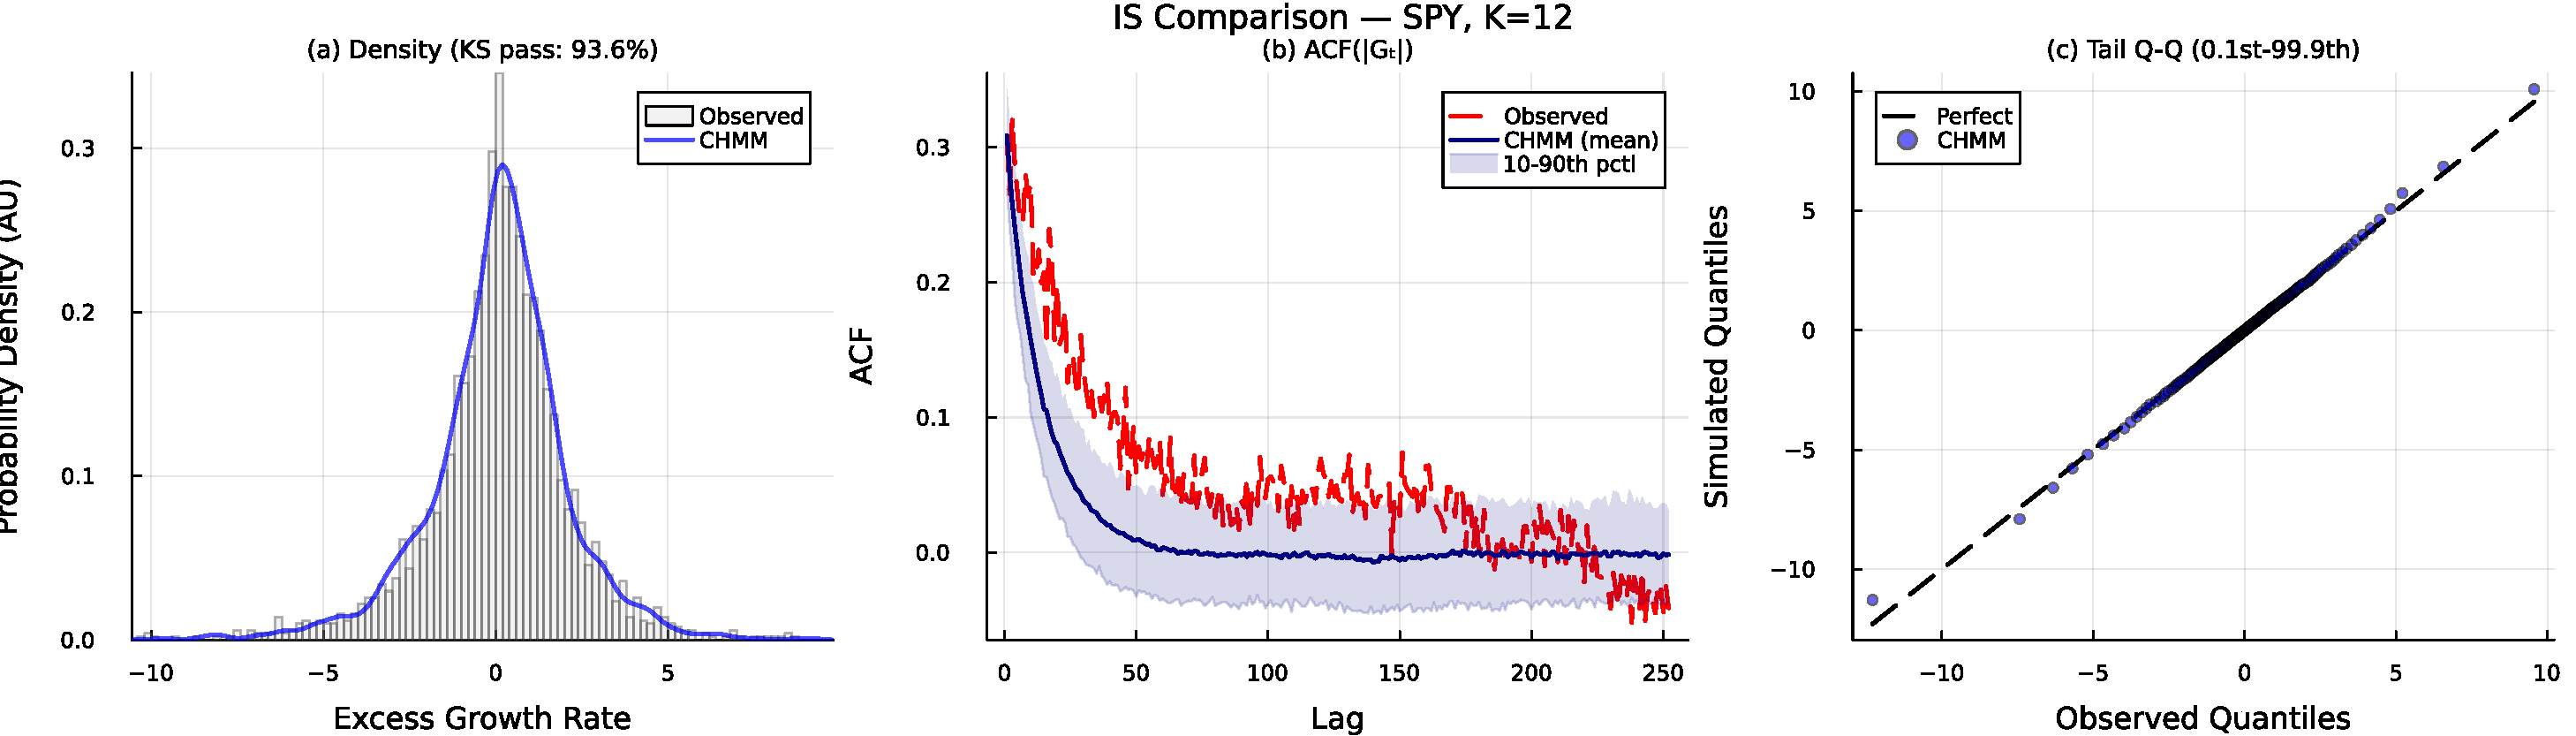
\includegraphics[width=\textwidth]{sections/figs/Fig-3-IS-Comparison-K12.pdf}
    \caption{$K = 12$}
\end{subfigure}
\hfill
\begin{subfigure}[b]{0.32\textwidth}
    
\includegraphics[width=\textwidth]{sections/figs/Fig-3-IS-Comparison-K15.pdf}
    \caption{$K = 15$}
\end{subfigure}
\hfill
\begin{subfigure}[b]{0.32\textwidth}
    
\includegraphics[width=\textwidth]{sections/figs/Fig-3-IS-Comparison-K21.pdf}
    \caption{$K = 21$}
\end{subfigure}
\caption{In-sample CHMM comparison panels at the non-selected state resolutions. Panel $K = 18$ is reproduced in Figure~\ref{fig:is_comparison} of the main text.}
\label{fig:k_sweep_panels_is}
\end{figure}

\subsection{Out-of-Sample Validation at Non-Selected State Resolutions}

Figure~\ref{fig:k_sweep_panels_oos} shows the out-of-sample validation panels for $K \in \{3, 6, 9, 12, 15, 21\}$.
KS pass rates remain above 91\% at all resolutions; the $K = 18$ panel is reproduced in Figure~\ref{fig:oos_validation} of the main text.

\begin{figure}[H]
\centering
\begin{subfigure}[b]{0.32\textwidth}
    
\includegraphics[width=\textwidth]{sections/figs/Fig-4-OoS-Validation-K3.pdf}
    \caption{$K = 3$}
\end{subfigure}
\hfill
\begin{subfigure}[b]{0.32\textwidth}
    
\includegraphics[width=\textwidth]{sections/figs/Fig-4-OoS-Validation-K6.pdf}
    \caption{$K = 6$}
\end{subfigure}
\hfill
\begin{subfigure}[b]{0.32\textwidth}
    
\includegraphics[width=\textwidth]{sections/figs/Fig-4-OoS-Validation-K9.pdf}
    \caption{$K = 9$}
\end{subfigure}

\vspace{0.4cm}

\begin{subfigure}[b]{0.32\textwidth}
    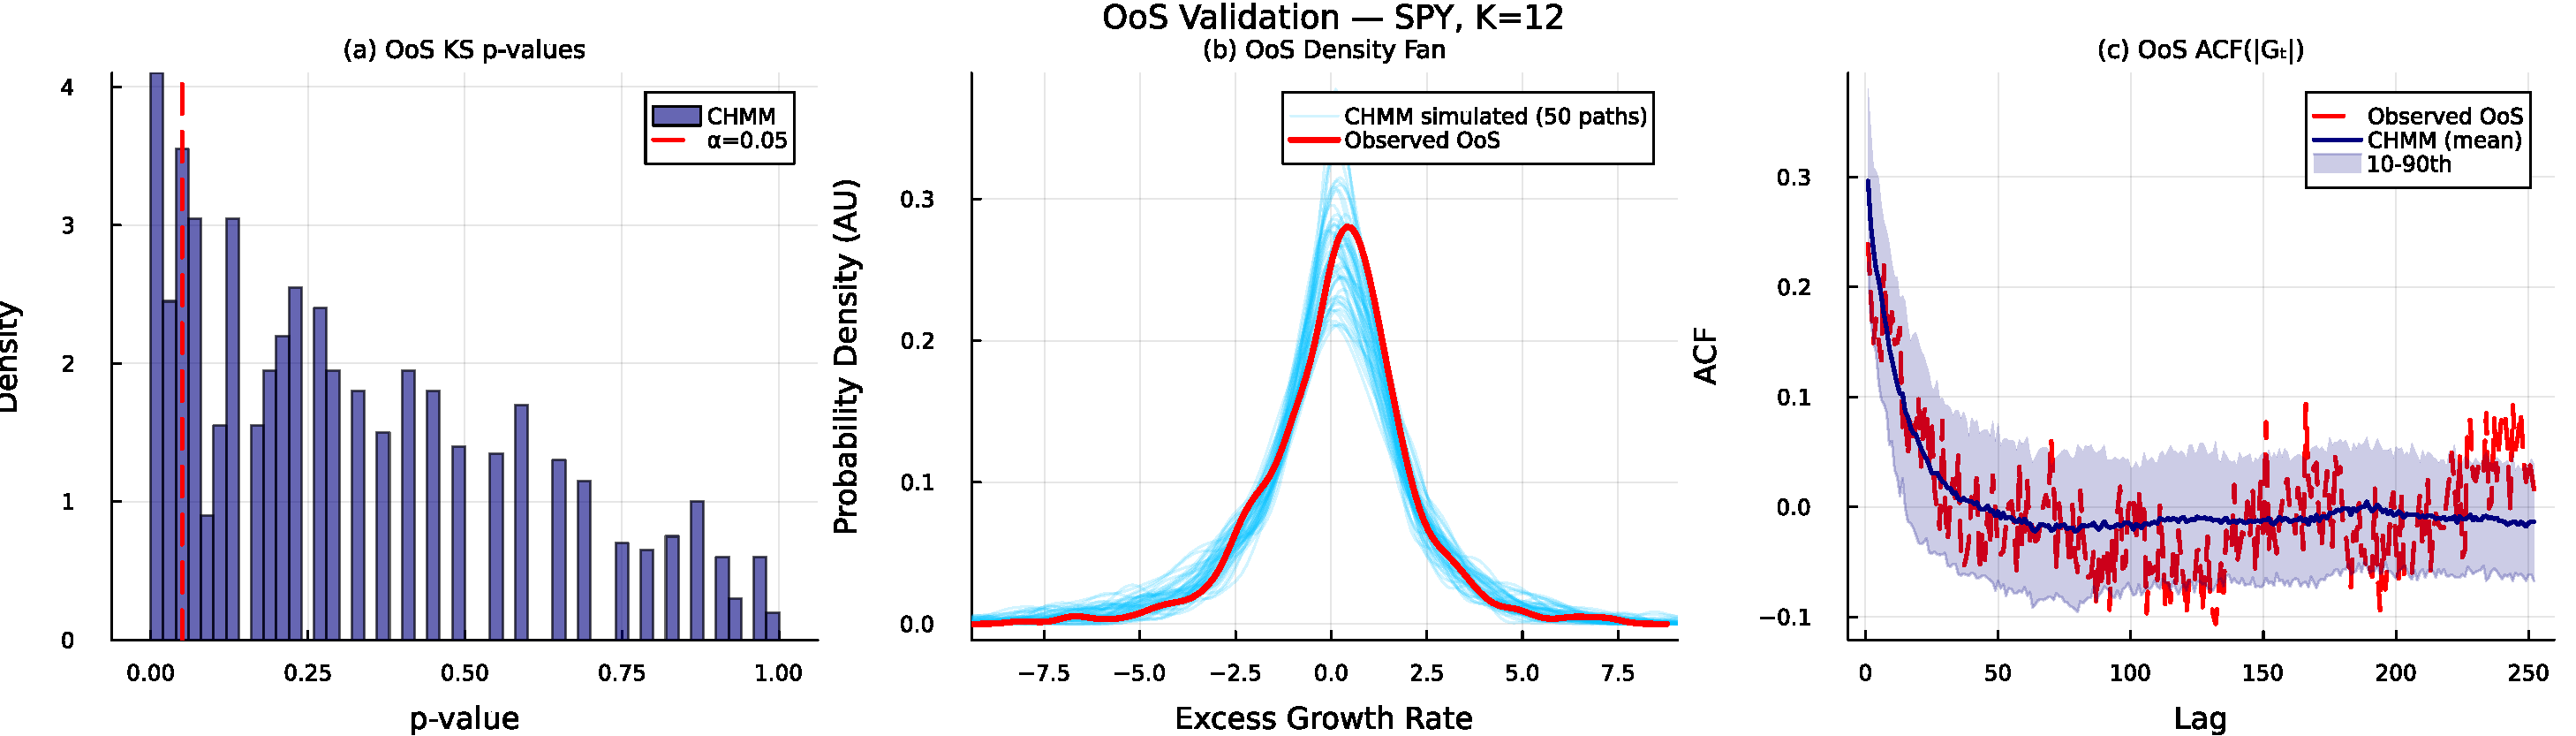
\includegraphics[width=\textwidth]{sections/figs/Fig-4-OoS-Validation-K12.pdf}
    \caption{$K = 12$}
\end{subfigure}
\hfill
\begin{subfigure}[b]{0.32\textwidth}
    
\includegraphics[width=\textwidth]{sections/figs/Fig-4-OoS-Validation-K15.pdf}
    \caption{$K = 15$}
\end{subfigure}
\hfill
\begin{subfigure}[b]{0.32\textwidth}
    
\includegraphics[width=\textwidth]{sections/figs/Fig-4-OoS-Validation-K21.pdf}
    \caption{$K = 21$}
\end{subfigure}
\caption{Out-of-sample CHMM validation panels at the non-selected state resolutions.}
\label{fig:k_sweep_panels_oos}
\end{figure}

\subsection{ACF Comparison Across State Resolutions}

Figure~\ref{fig:acf_all} shows the ACF of $|G_t|$ for the CHMM at $K = 3$, $K = 12$, and $K = 18$, compared to the observed ACF.
At all resolutions, the simulated ACF (shown as the median with 10th--90th percentile envelope across 1{,}000 paths) tracks the observed slow decay pattern.

\begin{figure}[H]
\centering
\begin{subfigure}[b]{0.32\textwidth}
    
\includegraphics[width=\textwidth]{sections/figs/Fig-ACF-Comparison-K3.pdf}
    \caption{$K = 3$}
\end{subfigure}
\hfill
\begin{subfigure}[b]{0.32\textwidth}
    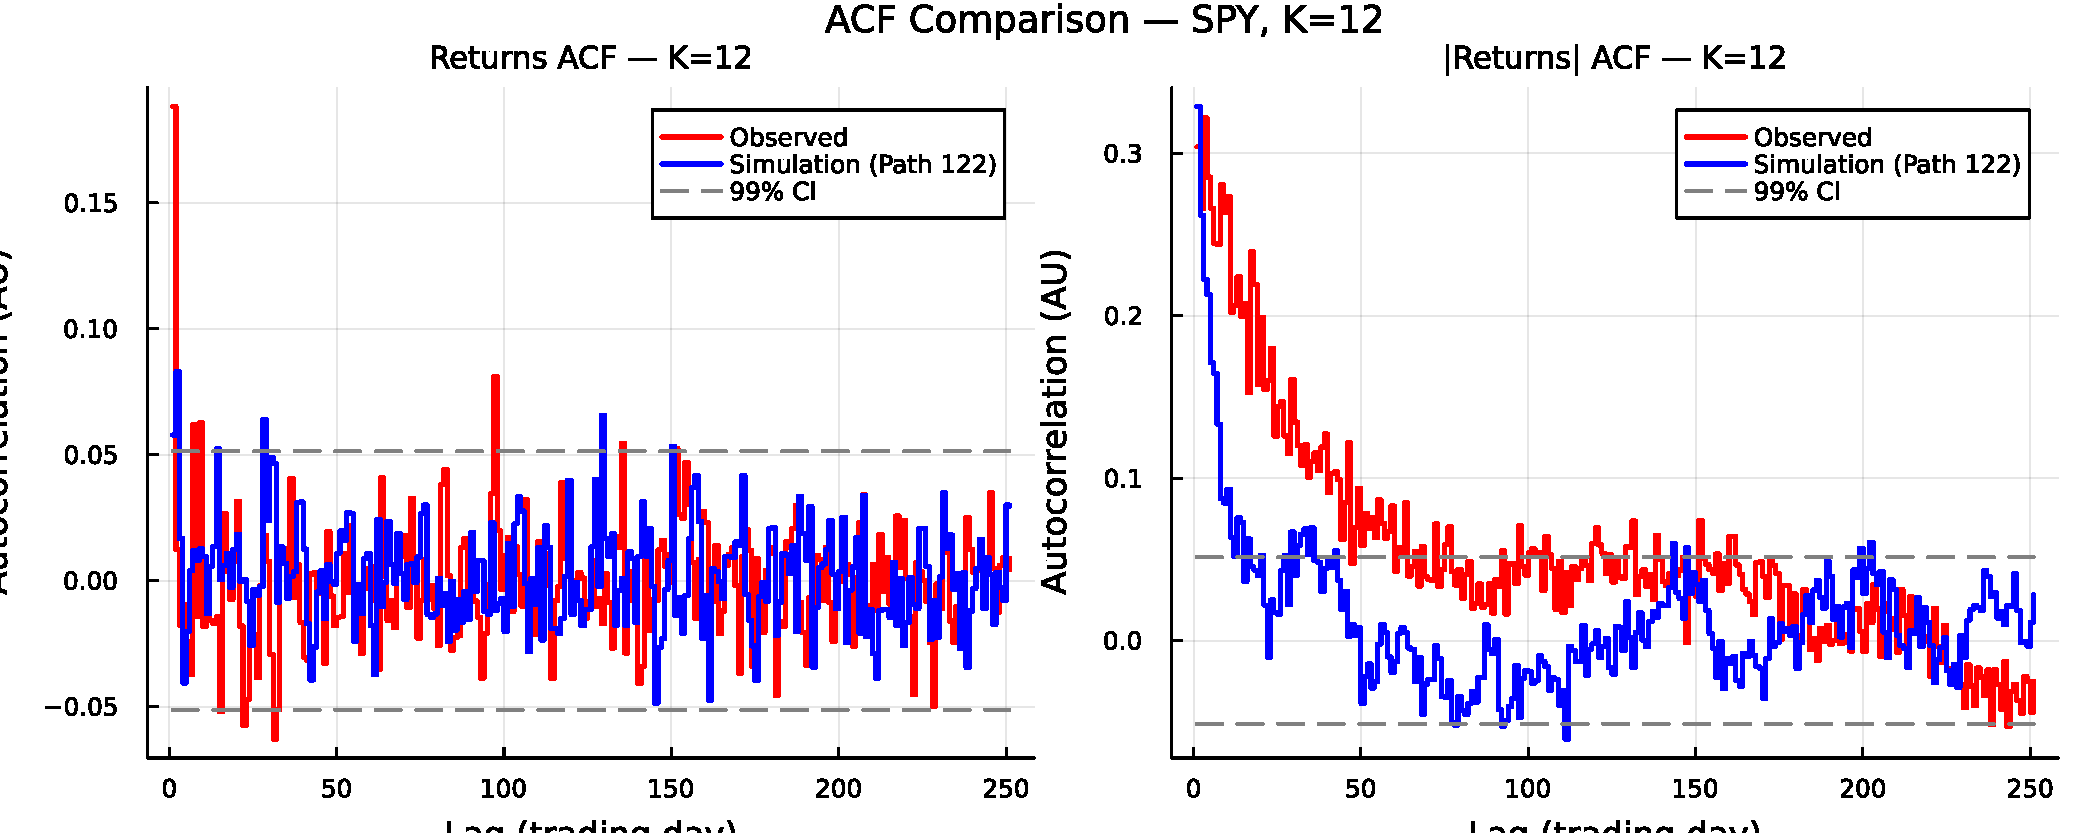
\includegraphics[width=\textwidth]{sections/figs/Fig-ACF-Comparison-K12.pdf}
    \caption{$K = 12$}
\end{subfigure}
\hfill
\begin{subfigure}[b]{0.32\textwidth}
    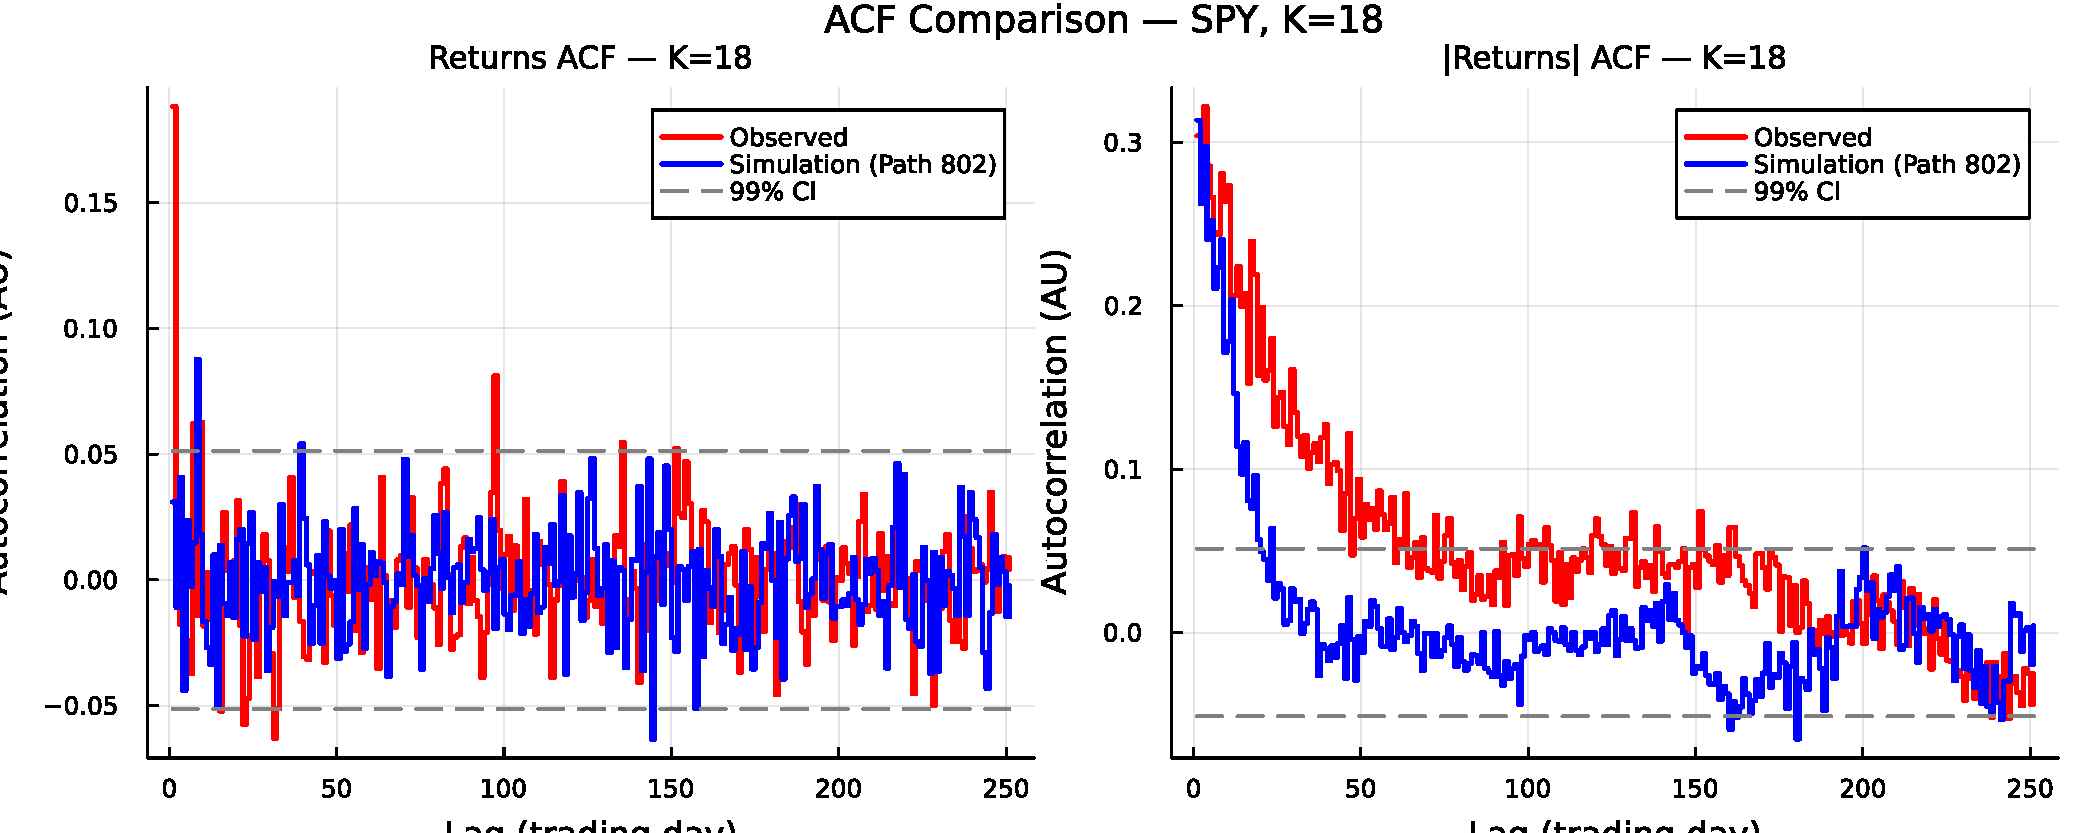
\includegraphics[width=\textwidth]{sections/figs/Fig-ACF-Comparison-K18.pdf}
    \caption{$K = 18$ (selected)}
\end{subfigure}
\caption{ACF of $|G_t|$ for the CHMM at $K = 3$, $K = 12$, and $K = 18$. The simulated 10th--90th percentile envelope (shaded) envelopes the observed ACF (red dashed), confirming that the CHMM reproduces volatility clustering without jump augmentation across the entire sweep.}
\label{fig:acf_all}
\end{figure}

\subsection{Example Simulated Trajectories}

Figure~\ref{fig:trajectories} shows example simulated return trajectories for $K = 6$ and $K = 18$, illustrating the qualitative dynamics produced by the CHMM.
Both trajectories exhibit the characteristic pattern of financial returns: extended periods of low volatility punctuated by clusters of large-magnitude events.

\begin{figure}[H]
\centering
\begin{subfigure}[b]{0.48\textwidth}
    
\includegraphics[width=\textwidth]{sections/figs/Fig-Trajectory-Example-K6.pdf}
    \caption{$K = 6$}
\end{subfigure}
\hfill
\begin{subfigure}[b]{0.48\textwidth}
    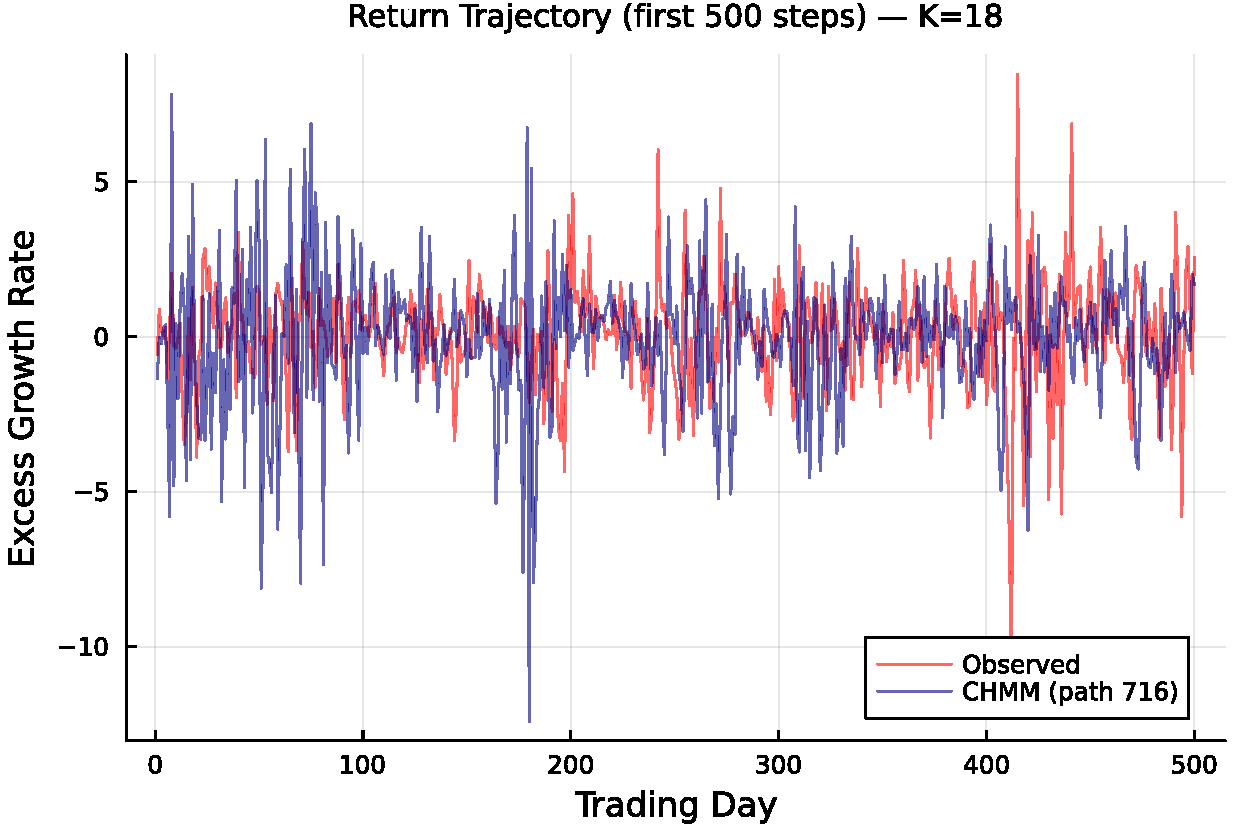
\includegraphics[width=\textwidth]{sections/figs/Fig-Trajectory-Example-K18.pdf}
    \caption{$K = 18$}
\end{subfigure}
\caption{Example simulated return trajectories. The alternation between calm (central states) and volatile (tail states) periods produces the volatility clustering characteristic of empirical financial returns.}
\label{fig:trajectories}
\end{figure}

\subsection{Multi-Emission Figures at $K = 18$}
\label{sec:multi_emission_figs}

This appendix reproduces the standard diagnostic suite (emission PDFs, transition matrix, stationary distribution, residence times, IS comparison, OoS validation, and convergence) for the two heavy-tailed emission families (CHMM-t and CHMM-L) at the selected state resolution $K = 18$.
The Gaussian counterparts are already shown as Figures~\ref{fig:model_internals},~\ref{fig:is_comparison},~\ref{fig:oos_validation},~\ref{fig:convergence_all},~\ref{fig:transition_all},~\ref{fig:stationary_all}, and~\ref{fig:residence_all} in the main text and above in this appendix.
The figures confirm that the shared forward--backward scaffold produces internally-similar regime structure across the three families: the near-diagonal transition band, the $K$-component dense emission cover, the longer central-state residence times, and the monotone log-likelihood convergence are features of the CHMM framework and not of the Gaussian component specifically.

\paragraph{Emission PDFs.}
Figure~\ref{fig:emissions_families} compares the learned $K = 18$ emissions for the three families.
The CHMM-t panel's per-state $\nu_k$ allocation is visible in the narrower modes of certain tail states; the CHMM-L panel's Laplace components have sharper peaks and slower exponential tail decay than the Gaussians.

\begin{figure}[H]
\centering
\begin{subfigure}[b]{0.32\textwidth}
    
\includegraphics[width=\textwidth]{sections/figs/Fig-Emission-PDFs-K18-N.pdf}
    \caption{CHMM-N (Gaussian)}
\end{subfigure}
\hfill
\begin{subfigure}[b]{0.32\textwidth}
    
\includegraphics[width=\textwidth]{sections/figs/Fig-Emission-PDFs-K18-t.pdf}
    \caption{CHMM-t (Student-t)}
\end{subfigure}
\hfill
\begin{subfigure}[b]{0.32\textwidth}
    
\includegraphics[width=\textwidth]{sections/figs/Fig-Emission-PDFs-K18-L.pdf}
    \caption{CHMM-L (Laplace)}
\end{subfigure}
\caption{Learned emission distributions at $K = 18$ across the three emission families, overlaid on the observed SPY return histogram. Heavier-tailed emission families (t, L) give individual components more tail mass, which is what closes the kurtosis gap of the Gaussian CHMM.}
\label{fig:emissions_families}
\end{figure}

\paragraph{Transition matrices.}
Figure~\ref{fig:transition_families} shows the $K = 18$ transition matrices learned by each family.
The near-diagonal band and the magnitude of self-transition probabilities are essentially unchanged across families, consistent with the ACF-MAE being stable across the family axis (Table~\ref{tab:sensitivity_multi}).

\begin{figure}[H]
\centering
\begin{subfigure}[b]{0.32\textwidth}
    
\includegraphics[width=\textwidth]{sections/figs/Fig-Transition-Matrix-K18-N.pdf}
    \caption{CHMM-N}
\end{subfigure}
\hfill
\begin{subfigure}[b]{0.32\textwidth}
    
\includegraphics[width=\textwidth]{sections/figs/Fig-Transition-Matrix-K18-t.pdf}
    \caption{CHMM-t}
\end{subfigure}
\hfill
\begin{subfigure}[b]{0.32\textwidth}
    
\includegraphics[width=\textwidth]{sections/figs/Fig-Transition-Matrix-K18-L.pdf}
    \caption{CHMM-L}
\end{subfigure}
\caption{Learned transition matrices at $K = 18$ in log$_{10}$ color scale. The diagonal-band structure is preserved across all three emission families.}
\label{fig:transition_families}
\end{figure}

\paragraph{Stationary distributions and residence times.}
Figure~\ref{fig:stationary_families} and Figure~\ref{fig:residence_families} compare the stationary distribution and natural residence times $\tau_k = 1/(1 - T_{kk})$ across families at $K = 18$.
The mass concentration at central states and the monotone decrease of $\tau_k$ toward the tails are features of the regime structure, not the emission family.

\begin{figure}[H]
\centering
\begin{subfigure}[b]{0.32\textwidth}
    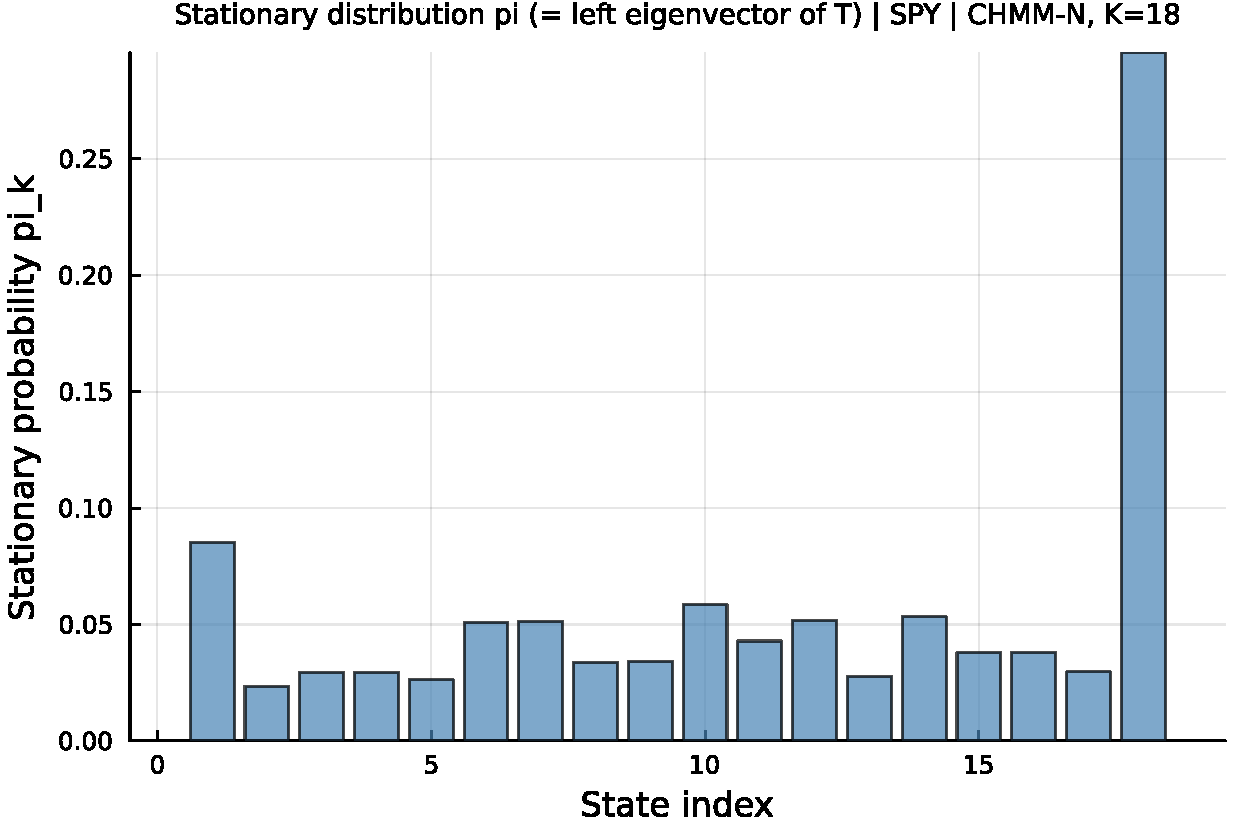
\includegraphics[width=\textwidth]{sections/figs/Fig-Stationary-Distribution-K18-N.pdf}
    \caption{CHMM-N}
\end{subfigure}
\hfill
\begin{subfigure}[b]{0.32\textwidth}
    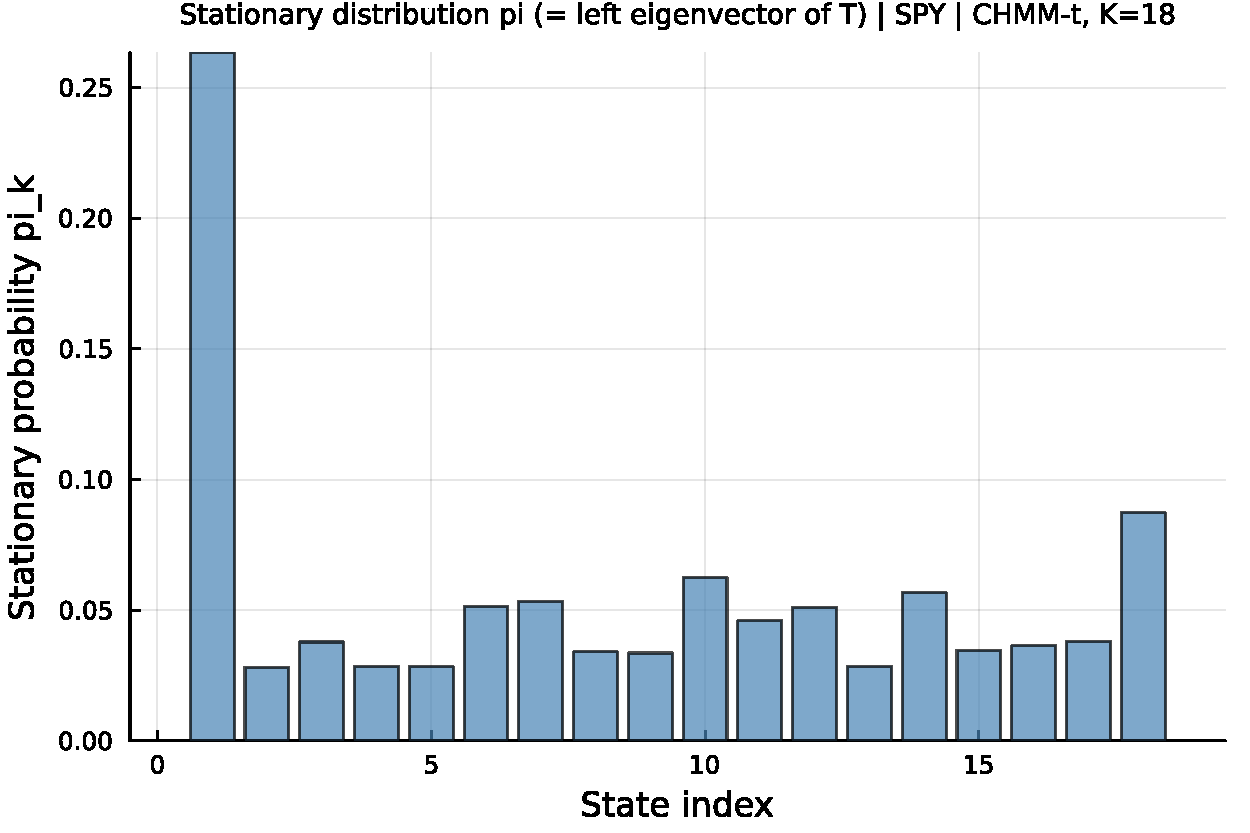
\includegraphics[width=\textwidth]{sections/figs/Fig-Stationary-Distribution-K18-t.pdf}
    \caption{CHMM-t}
\end{subfigure}
\hfill
\begin{subfigure}[b]{0.32\textwidth}
    
\includegraphics[width=\textwidth]{sections/figs/Fig-Stationary-Distribution-K18-L.pdf}
    \caption{CHMM-L}
\end{subfigure}
\caption{Stationary distributions $\bar{\boldsymbol{\pi}}$ at $K = 18$ across the three emission families.}
\label{fig:stationary_families}
\end{figure}

\begin{figure}[H]
\centering
\begin{subfigure}[b]{0.32\textwidth}
    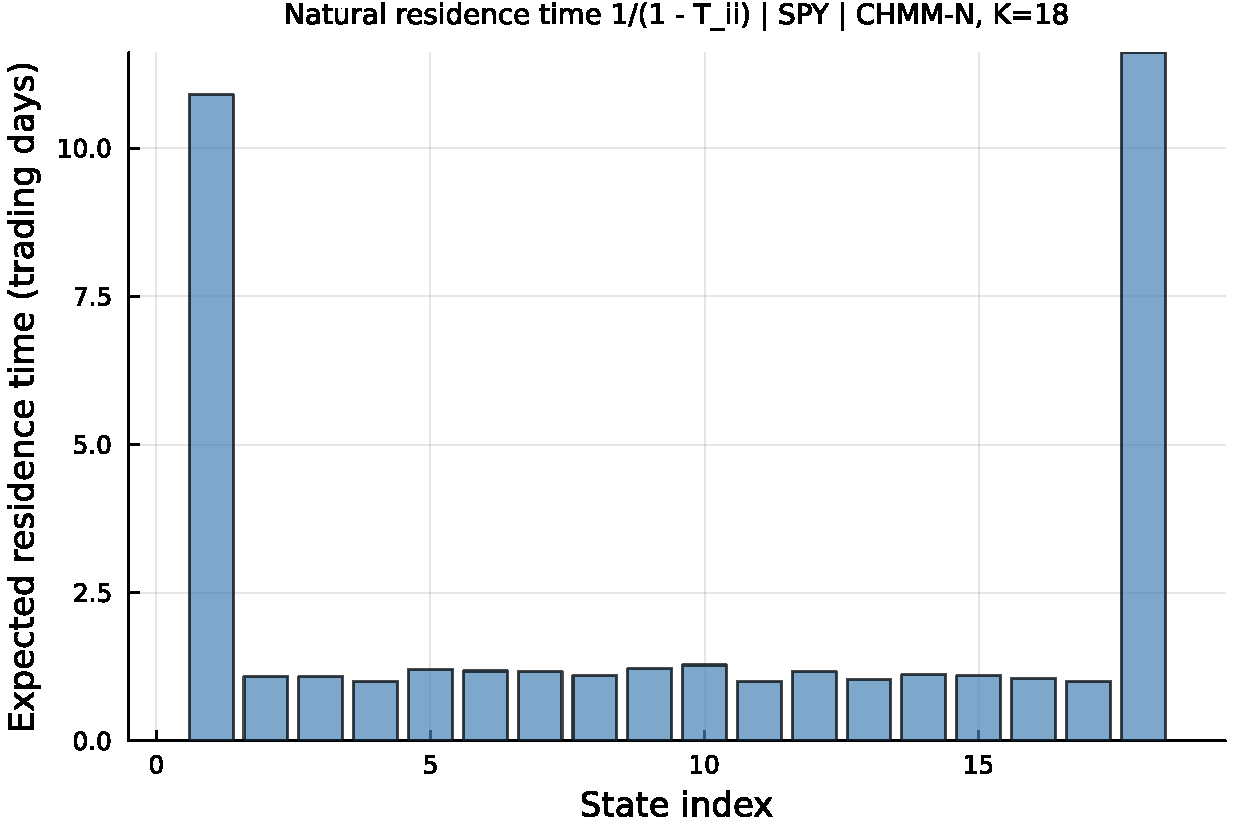
\includegraphics[width=\textwidth]{sections/figs/Fig-Residence-Times-K18-N.pdf}
    \caption{CHMM-N}
\end{subfigure}
\hfill
\begin{subfigure}[b]{0.32\textwidth}
    
\includegraphics[width=\textwidth]{sections/figs/Fig-Residence-Times-K18-t.pdf}
    \caption{CHMM-t}
\end{subfigure}
\hfill
\begin{subfigure}[b]{0.32\textwidth}
    
\includegraphics[width=\textwidth]{sections/figs/Fig-Residence-Times-K18-L.pdf}
    \caption{CHMM-L}
\end{subfigure}
\caption{Natural residence times $\tau_k = 1/(1 - T_{kk})$ at $K = 18$ across the three emission families.}
\label{fig:residence_families}
\end{figure}

\paragraph{In-sample comparison.}
Figure~\ref{fig:is_families} reproduces the three-panel in-sample comparison (density, ACF of $|G_t|$, tail Q-Q) at $K = 18$ for the two heavy-tailed families; the CHMM-N panel is Figure~\ref{fig:is_comparison} in the main text.

\begin{figure}[H]
\centering
\begin{subfigure}[b]{0.48\textwidth}
    
\includegraphics[width=\textwidth]{sections/figs/Fig-3-IS-Comparison-K18-t.pdf}
    \caption{CHMM-t}
\end{subfigure}
\hfill
\begin{subfigure}[b]{0.48\textwidth}
    
\includegraphics[width=\textwidth]{sections/figs/Fig-3-IS-Comparison-K18-L.pdf}
    \caption{CHMM-L}
\end{subfigure}
\caption{In-sample model comparison at $K = 18$ for the two heavy-tailed emission families. Each panel shows (a) marginal density with KS pass rate, (b) ACF of $|G_t|$, and (c) tail Q-Q plot. The CHMM-N counterpart is Figure~\ref{fig:is_comparison}.}
\label{fig:is_families}
\end{figure}

\paragraph{Out-of-sample validation.}
Figure~\ref{fig:oos_families} shows the OoS validation panels for CHMM-t and CHMM-L at $K = 18$.
The CHMM-t panel demonstrates the OoS kurtosis alignment noted in the main text (simulated 6.40 vs.\ observed 6.24), and the CHMM-L panel shows the tighter density fan produced by the heavier Laplace tails relative to the Gaussian.

\begin{figure}[H]
\centering
\begin{subfigure}[b]{0.48\textwidth}
    
\includegraphics[width=\textwidth]{sections/figs/Fig-4-OoS-Validation-K18-t.pdf}
    \caption{CHMM-t}
\end{subfigure}
\hfill
\begin{subfigure}[b]{0.48\textwidth}
    
\includegraphics[width=\textwidth]{sections/figs/Fig-4-OoS-Validation-K18-L.pdf}
    \caption{CHMM-L}
\end{subfigure}
\caption{Out-of-sample validation at $K = 18$ for the two heavy-tailed emission families. Each panel shows (a) KS $p$-values, (b) OoS density fan, and (c) OoS ACF of $|G_t|$. The CHMM-N counterpart is Figure~\ref{fig:oos_validation}.}
\label{fig:oos_families}
\end{figure}

\paragraph{Convergence.}
Figure~\ref{fig:convergence_families} shows the Baum-Welch / ECM / weighted-EM log-likelihood histories at $K = 18$ for all three families.
The CHMM-t and CHMM-L curves inherit the monotone increase of the classical EM guarantee; the CHMM-t curve has a slightly longer pre-plateau phase because each ECM sub-iteration refines $\nu_k$ with a golden-section search.

\begin{figure}[H]
\centering
\begin{subfigure}[b]{0.32\textwidth}
    
\includegraphics[width=\textwidth]{sections/figs/Fig-Convergence-K18-N.pdf}
    \caption{CHMM-N}
\end{subfigure}
\hfill
\begin{subfigure}[b]{0.32\textwidth}
    
\includegraphics[width=\textwidth]{sections/figs/Fig-Convergence-K18-t.pdf}
    \caption{CHMM-t}
\end{subfigure}
\hfill
\begin{subfigure}[b]{0.32\textwidth}
    
\includegraphics[width=\textwidth]{sections/figs/Fig-Convergence-K18-L.pdf}
    \caption{CHMM-L}
\end{subfigure}
\caption{Log-likelihood histories at $K = 18$ across the three emission families. All three curves are monotonically non-decreasing and plateau well before the $\texttt{max\_iter} = 60$ budget.}
\label{fig:convergence_families}
\end{figure}

\subsection{Cross-Asset Dependence Models: Derivations and Diagnostics}
\label{sec:cross_asset_supp}

This appendix provides the technical background for the SIM and copula constructions used in Section~\ref{sec:cross_asset} of the main text.

\paragraph{Sklar's theorem and the rank-reordering simulator.}
Sklar's theorem \cite{sklar1959fonctions, nelsen2006introduction} states that any $d$-dimensional joint CDF $H(g_1, \dots, g_d)$ with continuous marginals $F_1, \dots, F_d$ can be written as $H = C(F_1, \dots, F_d)$ for a unique copula $C$.
The rank-reordering simulator exploits this uniqueness.
If $\tilde{\mathbf{G}}$ is a matrix whose $j$-th column is an i.i.d.\ sample from $F_j$, and $\mathbf{U}$ is an independent sample from $C$, then reordering each column of $\tilde{\mathbf{G}}$ so that its ranks match $\mathbf{U}$'s produces a sample from $H$, up to discrete approximation error in the empirical ranks.
Crucially, reordering never creates new values: each column of the output is a permutation of the corresponding column of $\tilde{\mathbf{G}}$, so marginal distributions are preserved exactly \cite{iman1982distribution}.

\paragraph{Kendall's $\tau$ inversion.}
Given in-sample returns $\mathbf{R} \in \mathbb{R}^{T \times d}$, we estimate the pairwise Kendall's $\tau_{ij}$ from concordant/discordant pair counts and invert to the correlation scale via the analytic relationship $\rho_{ij} = \sin(\pi \tau_{ij} / 2)$, which holds exactly for the Gaussian copula family and is commonly used as a robust correlation estimator for the Student-t copula \cite{embrechts2002correlation, mcneil2015quantitative}.
The resulting matrix $\hat{\Sigma}$ is symmetric but not guaranteed positive semi-definite; we project to the nearest PSD matrix by clipping negative eigenvalues to $10^{-8}$ and rescaling the diagonal to unity.

\paragraph{Profile MLE for $\nu$.}
The Student-t copula log-density at a single pseudo-uniform observation $\mathbf{u} \in [0,1]^d$, with $x_j = t_\nu^{-1}(u_j)$ and $\mathbf{x} = (x_1, \dots, x_d)^\top$, is
\begin{align}
    \log c_t(\mathbf{u}; \Sigma, \nu)
    \;=\;&
    \log \Gamma\!\left(\tfrac{\nu+d}{2}\right)
    + (d-1)\,\log \Gamma\!\left(\tfrac{\nu}{2}\right)
    - d\,\log \Gamma\!\left(\tfrac{\nu+1}{2}\right)
    - \tfrac{1}{2} \log |\Sigma|
    \notag \\
    &\;
    - \tfrac{\nu+d}{2}\,\log\!\left(1 + \tfrac{\mathbf{x}^{\!\top} \Sigma^{-1} \mathbf{x}}{\nu}\right)
    + \sum_{j=1}^{d} \tfrac{\nu+1}{2}\,\log\!\left(1 + \tfrac{x_j^2}{\nu}\right).
    \label{eq:tcop_ll}
\end{align}
Summing over $t = 1, \dots, T$ pseudo-observations yields the profile log-likelihood as a function of $\nu$ with $\Sigma$ held fixed at the Kendall's-$\tau$ estimate.
We evaluate equation~\eqref{eq:tcop_ll} on the discrete grid $\nu \in \{2, 3, 4, 5, 6, 8, 10, 15, 20, 30\}$ and select $\hat{\nu}$ as the grid point with the largest total log-likelihood.
In Section~\ref{sec:cross_asset} the selected value was $\hat{\nu} = 6$ on the six-asset universe.

\paragraph{Sampling the copula.}
To sample $T$ rows from the $d$-dimensional Gaussian copula with correlation $\Sigma$, we (i) compute the Cholesky factor $\Sigma = L L^\top$, (ii) draw $Z \sim \mathcal{N}(0, I_d)$ i.i.d.\ and form $Y = L Z$, and (iii) return $U = \Phi(Y)$ componentwise.
For the Student-t copula with degrees of freedom $\nu$, we draw $W \sim \chi^2_\nu / \nu$ independent of $Y$ and form the multivariate-$t$ variate $X = Y / \sqrt{W}$, then return $U = t_\nu(X)$ componentwise.

\paragraph{SIM regression summary.}
Table~\ref{tab:sim_regression} reports the fitted SIM regression coefficients and goodness-of-fit statistics for the non-market assets in Section~\ref{sec:cross_asset}.
QQQ's high $R^2 = 0.841$ reflects that the Nasdaq-100 ETF is essentially a linear combination of large-cap technology names that also drive the S\&P~500 index, while JNJ's lower $R^2 = 0.225$ reflects the limited systematic exposure of low-beta healthcare stocks.
These factor loadings and residual magnitudes are what the SIM simulation in equation~\eqref{eq:sim_sim} re-injects at simulation time, and they explain the uneven per-asset KS pass rates reported in Table~\ref{tab:cross_asset_sim_copula}.

\begin{table}[H]
\centering
\caption{SIM regression $\hat{G}_{j,t} = \hat{\alpha}_j + \hat{\beta}_j G_{\text{SPY},t} + \hat{\eta}_{j,t}$ for the five non-market assets, fitted on the 2014--2024 in-sample window ($T = 2{,}766$). Coefficients $\hat{\alpha}, \hat{\beta}$ and $R^2$ are reported for the factor equation used in equation~\eqref{eq:sim_sim}.}
\label{tab:sim_regression}
\small
\begin{tabular}{l ccc}
\toprule
Ticker & $\hat{\alpha}$ & $\hat{\beta}$ & $R^2$ \\
\midrule
NVDA & $0.347$   & $1.749$ & $0.370$ \\
JNJ  & $-0.016$  & $0.539$ & $0.225$ \\
JPM  & $0.001$   & $1.204$ & $0.483$ \\
AAPL & $0.106$   & $1.194$ & $0.474$ \\
QQQ  & $0.041$   & $1.134$ & $0.841$ \\
\bottomrule
\end{tabular}
\end{table}

\subsection{VIX Results Detail}

The CHMM framework was applied to VIX daily log returns to test generalization beyond equity returns.
VIX returns exhibit positive skewness (reflecting asymmetric volatility spikes), pronounced mean reversion, and extreme excess kurtosis, properties that differ fundamentally from equity returns.

The CHMM captured these properties effectively: at higher state resolutions ($K \geq 9$), the model achieved IS KS pass rates above 99\%, demonstrating that the Gaussian mixture mechanism can approximate even the positively skewed, heavy-tailed marginal distribution of VIX returns.
The regime decomposition provided by the Viterbi algorithm aligned with known market events, assigning high-volatility states to crisis episodes and low-volatility states to calm market periods.

The VIX extension demonstrates that the CHMM framework is not limited to equity returns but applies more broadly to financial time series with regime-switching dynamics, including volatility measures used directly as synthetic-data targets.

\subsection{Algorithm Descriptions}
\label{sec:algorithms}

This section provides detailed pseudocode for the main algorithms used in this study.
Algorithm~\ref{alg:chmm_em} is the unified EM procedure shared across all three emission families.
It makes explicit the \emph{shared scaffold} (quantile-based initialization, log-space forward-backward, transition update) and the three \emph{family-specific branches} (Gaussian M-step for CHMM-N, ECM with one-dimensional golden-section $\nu$-search for CHMM-t, closed-form weighted-median + weighted-MAD for CHMM-L); the branch points are lines~\ref{line:init}, \ref{line:emit}, and \ref{line:mstep}.
Visualizing the three variants as a single algorithm with three M-step branches makes the architectural contribution of the paper --- one EM engine, three interchangeable emission families --- immediate from the pseudocode.
Algorithm~\ref{alg:viterbi} presents the Viterbi algorithm for decoding the most likely hidden state sequence.
Algorithm~\ref{alg:chmm_simulate} describes the CHMM simulation procedure for generating synthetic return paths.
Algorithm~\ref{alg:copula_sim} describes the cross-asset rank-reordering simulator for copula-based multi-asset synthesis.
Algorithm~\ref{alg:sim_build} details the SIM regression-and-resampling pipeline.

% ========================================================================================= %
% Algorithm 1: Baum-Welch (EM) for Continuous Gaussian HMM
% ========================================================================================= %
% Unified EM algorithm with family-specific M-step switch
% ========================================================================================= %
\begin{algorithm}[tp]
\caption{Unified EM algorithm for the CHMM family. Lines~\ref{line:init}, \ref{line:emit}, and \ref{line:mstep} branch on the emission family $F \in \{\mathcal{N}, t, L\}$; every other line is identical across families. CHMM-N and CHMM-L instantiate classical EM; CHMM-t instantiates an ECM sequence whose second CM step updates $\nu_k$ by a one-dimensional golden-section search on the per-state $Q$-function.}
\label{alg:chmm_em}
\small
\begin{algorithmic}[1]
\REQUIRE Observations $O_{1:T}$, number of states $K$, tolerance $\text{tol}$, $\texttt{max\_iter}$, emission family $F \in \{\mathcal{N}, t, L\}$, if $F = t$ bracket $(\nu_{\min}, \nu_{\max})$ and initial $\nu^{(0)}$.
\ENSURE Transition matrix $\mathbf{T}$, per-state emission parameters $\boldsymbol\theta_{1:K}$, initial distribution $\boldsymbol{\pi}$.

\STATE \textbf{Quantile-Based Initialization.}
\STATE Sort $O^{(\text{sort})} \leftarrow \text{sort}(O_{1:T})$ and partition into $K$ equal chunks $\{C_1,\ldots,C_K\}$.
\FOR{$k = 1$ to $K$} \label{line:init}
    \STATE \textbf{switch} $F$
    \STATE \quad $F = \mathcal{N}$: $\mu_k \leftarrow \text{mean}(C_k)$, \quad $\sigma_k \leftarrow \max(\text{std}(C_k), 10^{-6})$.
    \STATE \quad $F = t$: $\mu_k \leftarrow \text{mean}(C_k)$, \quad $\sigma_k \leftarrow \max(\text{std}(C_k), 10^{-6})$, \quad $\nu_k \leftarrow \nu^{(0)}$.
    \STATE \quad $F = L$: $\mu_k \leftarrow \text{median}(C_k)$, \quad $b_k \leftarrow \max(\text{mean}(|C_k - \mu_k|), 10^{-6})$.
\ENDFOR
\STATE $T_{ij} \leftarrow 1/K$; \quad $\pi_k \leftarrow 1/K$; \quad $\mathcal{L}_{\text{prev}} \leftarrow -\infty$.

\STATE \textbf{EM Loop.}
\FOR{$n = 1$ to $\texttt{max\_iter}$}

    \STATE \textbf{E-Step --- per-family emission log-likelihood.} \label{line:emit}
    \STATE \textbf{switch} $F$
    \STATE \quad $F = \mathcal{N}$: $\log B_{t,k} \leftarrow \log \mathcal{N}(O_t \mid \mu_k, \sigma_k^2)$.
    \STATE \quad $F = t$: $\log B_{t,k} \leftarrow \log t_{\nu_k}(O_t; \mu_k, \sigma_k)$.
    \STATE \quad $F = L$: $\log B_{t,k} \leftarrow -\log(2 b_k) - |O_t - \mu_k|/b_k$.

    \STATE \textbf{E-Step --- shared log-space forward-backward.}
    \STATE $\log \alpha_1(k) \leftarrow \log \pi_k + \log B_{1,k}$.
    \FOR{$t = 2$ to $T$, $j = 1$ to $K$}
        \STATE $\log \alpha_t(j) \leftarrow \underset{i}{\text{logsumexp}}\!\left(\log \alpha_{t-1}(i) + \log T_{ij}\right) + \log B_{t,j}$.
    \ENDFOR
    \STATE $\log \beta_T(k) \leftarrow 0$.
    \FOR{$t = T-1$ down to $1$, $i = 1$ to $K$}
        \STATE $\log \beta_t(i) \leftarrow \underset{j}{\text{logsumexp}}\!\left(\log T_{ij} + \log B_{t+1,j} + \log \beta_{t+1}(j)\right)$.
    \ENDFOR
    \STATE Compute $\gamma_t(k)$ and $\xi_t(i,j)$ from equation~\eqref{eq:gamma_xi}.

    \STATE \textbf{Shared transition update.} $T_{ij} \leftarrow \sum_t \xi_t(i,j) \;/\; \sum_t \gamma_t(i)$; $\pi_k \leftarrow \gamma_1(k)$.

    \STATE \textbf{M-Step --- per-family emission update.} \label{line:mstep}
    \STATE \textbf{switch} $F$
    \STATE \quad $F = \mathcal{N}$ \COMMENT{classical Baum-Welch \citep{baum1970maximization}.}
    \STATE \qquad $\mu_k \leftarrow \sum_t \gamma_t(k)\, O_t / \sum_t \gamma_t(k)$.
    \STATE \qquad $\sigma_k \leftarrow \max\!\left(\sqrt{\sum_t \gamma_t(k) (O_t - \mu_k)^2 / \sum_t \gamma_t(k)},\; 10^{-6}\right)$.
    \STATE \quad $F = t$ \COMMENT{ECM of \citet{peel2000robust, liu1995ml}; closed-form $(\mu_k, \sigma_k)$ given $\nu_k$, then 1D search on $\nu_k$.}
    \STATE \qquad $u_{t,k} \leftarrow (\nu_k + 1) / (\nu_k + ((O_t - \mu_k)/\sigma_k)^2)$ for all $t, k$.
    \STATE \qquad $\mu_k \leftarrow \sum_t \gamma_t(k)\, u_{t,k}\, O_t / \sum_t \gamma_t(k)\, u_{t,k}$.
    \STATE \qquad $\sigma_k \leftarrow \max\!\left(\sqrt{\sum_t \gamma_t(k)\, u_{t,k}\,(O_t - \mu_k)^2 / \sum_t \gamma_t(k)},\; 10^{-6}\right)$.
    \STATE \qquad $\nu_k \leftarrow \arg\max_{\nu \in [\nu_{\min}, \nu_{\max}]} \sum_t \gamma_t(k)\, \log t_\nu(O_t; \mu_k, \sigma_k)$ \COMMENT{40-iter golden-section search.}
    \STATE \quad $F = L$ \COMMENT{closed-form weighted Laplace MLE.}
    \STATE \qquad $\mu_k \leftarrow \text{WeightedMedian}(O_{1:T},\, \gamma_{1:T}(k))$ \COMMENT{cumulative-weight bracketing with interpolation at the $W_k/2$ crossing.}
    \STATE \qquad $b_k \leftarrow \max\!\left(\sum_t \gamma_t(k)\, |O_t - \mu_k| / \sum_t \gamma_t(k),\; 10^{-6}\right)$.

    \STATE \textbf{Convergence check.} $\mathcal{L}^{(n)} \leftarrow \underset{k}{\text{logsumexp}}(\log \alpha_T(k))$.
    \IF{$|\mathcal{L}^{(n)} - \mathcal{L}_{\text{prev}}| < \text{tol}$} \STATE \textbf{break} \ENDIF
    \STATE $\mathcal{L}_{\text{prev}} \leftarrow \mathcal{L}^{(n)}$.
\ENDFOR

\RETURN $\mathbf{T}, \boldsymbol\theta_{1:K}, \boldsymbol{\pi}$ \COMMENT{$\boldsymbol\theta_k = (\mu_k, \sigma_k)$ for $F = \mathcal{N}$; $(\mu_k, \sigma_k, \nu_k)$ for $F = t$; $(\mu_k, b_k)$ for $F = L$.}
\end{algorithmic}
\end{algorithm}

% Backward-compatibility labels: any older cross-reference to the separate algorithms now points at the unified block.
\newcommand{\algbaumwelch}{\ref{alg:chmm_em}}
\newcommand{\algecmstudentt}{\ref{alg:chmm_em}}
\newcommand{\algemlaplace}{\ref{alg:chmm_em}}

% ========================================================================================= %
% Algorithm 2: Viterbi Decoding
% ========================================================================================= %
\begin{algorithm}[tp]
\caption{Viterbi decoding for the most likely hidden state sequence}
\label{alg:viterbi}
\small
\begin{algorithmic}[1]
\REQUIRE Observations $O_{1:T}$, Trained CHMM $\mathcal{M} = (\mathbf{T}, \{\mu_k, \sigma_k\}, \boldsymbol{\pi})$
\ENSURE Most probable state sequence $S_{1:T}^*$

\FOR{$k = 1$ to $K$}
    \STATE $\log \delta_1(k) \leftarrow \log(1/K) + \log \mathcal{N}(O_1 \mid \mu_k, \sigma_k^2)$.
\ENDFOR

\FOR{$t = 2$ to $T$}
    \FOR{$j = 1$ to $K$}
        \STATE $\text{vals}(i) \leftarrow \log \delta_{t-1}(i) + \log T_{ij}$ for all $i$.
        \STATE $\log \delta_t(j) \leftarrow \max_i \text{vals}(i) + \log \mathcal{N}(O_t \mid \mu_j, \sigma_j^2)$.
        \STATE $\psi_t(j) \leftarrow \arg\max_i \text{vals}(i)$.
    \ENDFOR
\ENDFOR

\STATE $S_T^* \leftarrow \arg\max_k \log \delta_T(k)$.
\FOR{$t = T-1$ down to $1$}
    \STATE $S_t^* \leftarrow \psi_{t+1}(S_{t+1}^*)$.
\ENDFOR

\RETURN $S_{1:T}^*$
\end{algorithmic}
\end{algorithm}

% ========================================================================================= %
% Algorithm 3: CHMM Simulation
% ========================================================================================= %
\begin{algorithm}[tp]
\caption{CHMM simulation of synthetic excess growth rate paths}
\label{alg:chmm_simulate}
\small
\begin{algorithmic}[1]
\REQUIRE Trained CHMM $\mathcal{M} = (\mathbf{T}, \{\mu_k, \sigma_k\}, \boldsymbol{\pi})$, Number of steps $M$, Number of paths $P$
\ENSURE Simulated return paths $\{\hat{G}^{(p)}_{1:M}\}_{p=1}^{P}$

\FOR{$p = 1$ to $P$}
    \STATE Sample initial state $S_1 \sim \text{Categorical}(\boldsymbol{\pi})$.
    \FOR{$t = 1$ to $M$}
        \STATE Emit observation $\hat{G}_t^{(p)} \sim \mathcal{N}(\mu_{S_t}, \sigma_{S_t}^2)$.
        \IF{$t < M$}
            \STATE Transition to next state $S_{t+1} \sim \text{Categorical}(\mathbf{T}_{S_t, \cdot})$.
        \ENDIF
    \ENDFOR
\ENDFOR

\RETURN $\{\hat{G}^{(p)}_{1:M}\}_{p=1}^{P}$
\end{algorithmic}
\end{algorithm}

% ========================================================================================= %
% Algorithm 4: Cross-Asset Copula Rank Reordering Simulation
% ========================================================================================= %
\begin{algorithm}[tp]
\caption{Cross-asset copula simulation via rank reordering}
\label{alg:copula_sim}
\small
\begin{algorithmic}[1]
\REQUIRE Fitted per-asset CHMMs $\{\mathcal{M}_j\}_{j=1}^d$, correlation matrix $\Sigma$ (PSD, unit diagonal), copula family $\mathcal{C} \in \{\text{Gaussian}, t_\nu\}$, path length $T$, number of paths $P$
\ENSURE Cross-asset path tensor $\{\hat{G}^{(p)}_{j,t}\}$ of shape $T \times d \times P$

\FOR{$p = 1$ to $P$}

    \STATE Draw copula sample $\mathbf{U}^{(p)} \in [0,1]^{T \times d}$ from $\mathcal{C}(\Sigma)$:
    \STATE \quad $L \leftarrow \text{Cholesky}(\Sigma)$, \; $Z \in \mathbb{R}^{T \times d} \sim \mathcal{N}(0, I_d)$ i.i.d.
    \STATE \quad $Y \leftarrow Z L^\top$
    \IF{$\mathcal{C} = $ Gaussian}
        \STATE \quad $\mathbf{U}^{(p)} \leftarrow \Phi(Y)$ componentwise
    \ELSE
        \STATE \quad Draw $W \sim \chi^2_\nu / \nu$ i.i.d. for $t = 1, \dots, T$; \; $X_{t,\cdot} \leftarrow Y_{t,\cdot} / \sqrt{W_t}$
        \STATE \quad $\mathbf{U}^{(p)} \leftarrow t_\nu(X)$ componentwise
    \ENDIF

    \FOR{$j = 1$ to $d$}
        \STATE Simulate $\tilde{g}_{j,1:T}^{(p)}$ from $\mathcal{M}_j$ via Algorithm~\ref{alg:chmm_simulate}.
        \STATE Compute order statistics $\tilde{g}_{j,(1)}^{(p)} \leq \cdots \leq \tilde{g}_{j,(T)}^{(p)}$.
        \STATE Compute ranks $r_{j,t}^{(p)} \leftarrow \text{rank}(U_{j,t}^{(p)})$ for $t = 1, \dots, T$.
        \STATE $\hat{G}_{j,t}^{(p)} \leftarrow \tilde{g}_{j,(r_{j,t}^{(p)})}^{(p)}$ for $t = 1, \dots, T$.
    \ENDFOR
\ENDFOR

\RETURN $\{\hat{G}^{(p)}_{j,t}\}$
\end{algorithmic}
\end{algorithm}

% ========================================================================================= %
% Algorithm 5: SIM fit and simulate
% ========================================================================================= %
\begin{algorithm}[tp]
\caption{Single Index Model (SIM) construction and simulation}
\label{alg:sim_build}
\small
\begin{algorithmic}[1]
\REQUIRE In-sample return matrix $\mathbf{R} \in \mathbb{R}^{T \times d}$, market-column index $m$, market CHMM $\mathcal{M}_m$, path length $T$, number of paths $P$
\ENSURE Cross-asset path tensor $\{\hat{G}^{(p)}_{j,t}\}$ of shape $T \times d \times P$

\STATE \textbf{OLS fit.} For $j \neq m$:
\STATE \quad $\hat{\beta}_j \leftarrow \text{Cov}(\mathbf{R}_{:,j}, \mathbf{R}_{:,m}) / \text{Var}(\mathbf{R}_{:,m})$
\STATE \quad $\hat{\alpha}_j \leftarrow \overline{\mathbf{R}_{:,j}} - \hat{\beta}_j \overline{\mathbf{R}_{:,m}}$
\STATE \quad $\hat{\eta}_{j,t} \leftarrow R_{t,j} - \hat{\alpha}_j - \hat{\beta}_j R_{t,m}$, \; $R^2_j \leftarrow 1 - \sum_t \hat{\eta}_{j,t}^2 / \sum_t (R_{t,j} - \overline{\mathbf{R}_{:,j}})^2$

\FOR{$p = 1$ to $P$}
    \STATE Simulate market path $G_{m,1:T}^{(p)}$ from $\mathcal{M}_m$ via Algorithm~\ref{alg:chmm_simulate}.
    \STATE $\hat{G}_{m,t}^{(p)} \leftarrow G_{m,t}^{(p)}$.
    \FOR{$j \neq m$}
        \STATE Draw residual indices $\{\iota_t\}_{t=1}^T \sim \text{Uniform}(\{1, \dots, T\})$.
        \STATE $\hat{G}_{j,t}^{(p)} \leftarrow \hat{\alpha}_j + \hat{\beta}_j G_{m,t}^{(p)} + \hat{\eta}_{j,\iota_t}$.
    \ENDFOR
\ENDFOR

\RETURN $\{\hat{G}^{(p)}_{j,t}\}$
\end{algorithmic}
\end{algorithm}


% =========================================================================== %
% v7 revision supplemental
% =========================================================================== %

\subsection{CHMM-t Degrees-of-Freedom Diagnostics}
\label{sec:nu_diagnostics}

This appendix backs the discussion in Section~\ref{sec:discussion} of the CHMM-t in-sample kurtosis overshoot.
Figure~\ref{fig:nu_hist} plots the per-state $\nu_k$ histogram for the $K = 18$ CHMM-t fit on SPY IS (seed = $20260420$).
Twelve of the eighteen states rest at the upper ECM bracket ($\nu_k = 50$), and only two states lie near the lower bracket ($\nu_2 = 2.35$, $\nu_4 = 2.82$).
The simulated in-sample mixture kurtosis of $12.60$ is driven by the posterior mass routed to those two very heavy-tailed states, not by a systemic collapse to the lower bracket.

\begin{figure}[h]
\centering
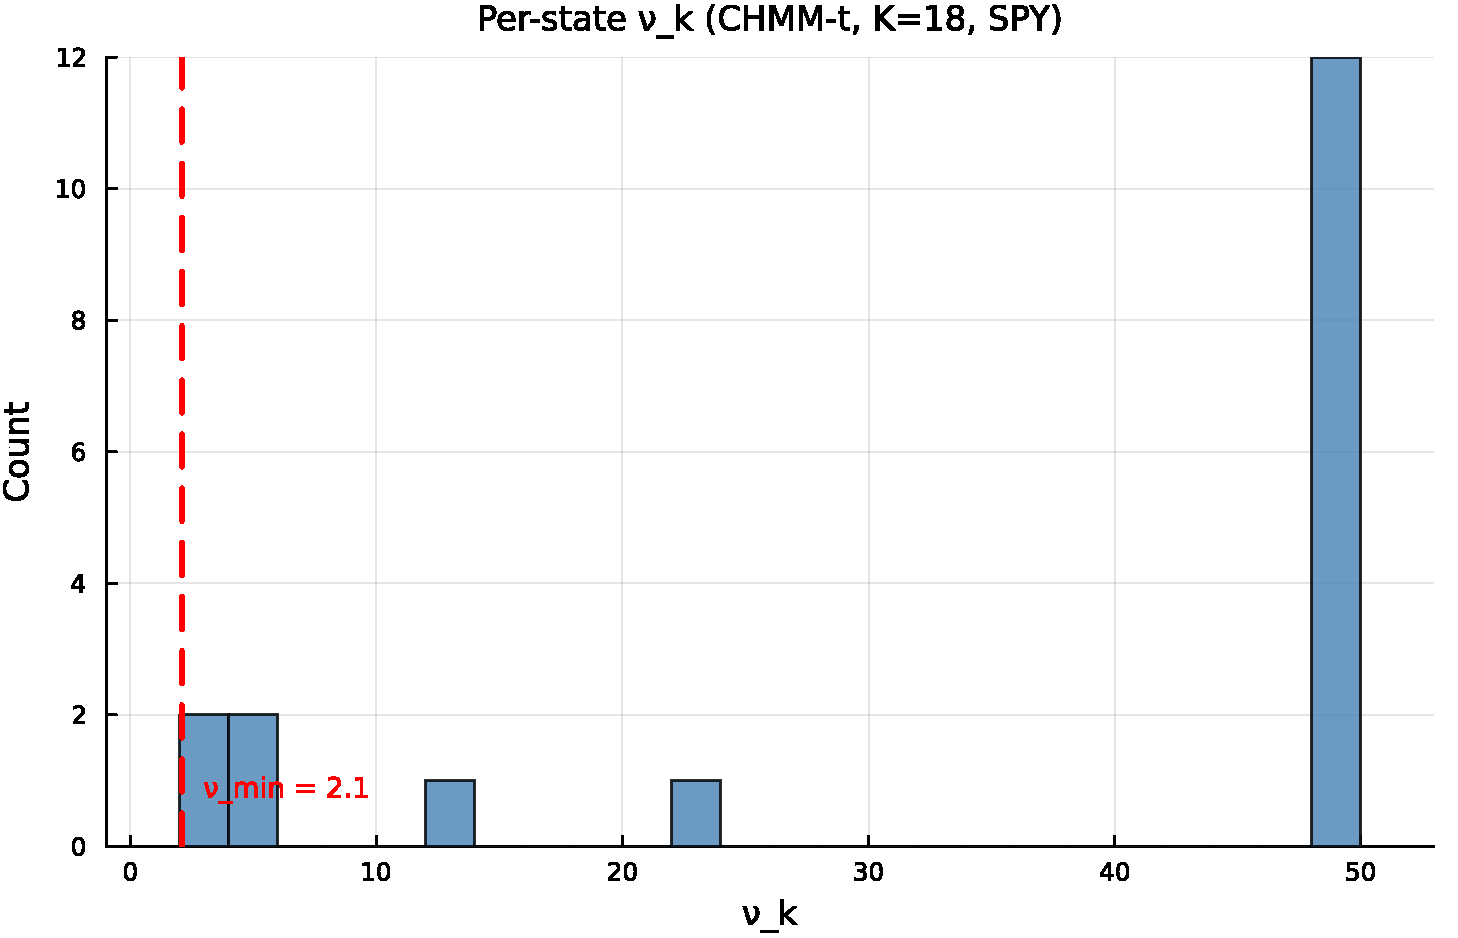
\includegraphics[width=0.75\textwidth]{sections/figs/Fig-v7-nu-Histogram.pdf}
\caption{Per-state degrees-of-freedom $\nu_k$ for the CHMM-t fit at $K = 18$ on SPY IS. The dashed red line marks the lower ECM bracket $\nu_{\min} = 2.1$. Only two states ($\nu_2 = 2.35$, $\nu_4 = 2.82$) sit near the lower bracket; the median $\nu_k$ is at the upper bracket.}
\label{fig:nu_hist}
\end{figure}

Table~\ref{tab:nu_bracket} reports the seven-metric panel for CHMM-t fits whose ECM bracket lower bound is lifted from $\nu_{\min} = 2.1$ through $\{2.5, 3.0, 4.0\}$, plus the Gaussian limit ($\nu = \infty$, equivalent to CHMM-N).
Lifting the bracket does not reduce the in-sample kurtosis overshoot: the simulated kurtosis moves within the $12.5$--$14.0$ band across bracket floors and only collapses to $5.05$ in the full Gaussian limit.
The overshoot is therefore a feature of the Student-t emission family at $K = 18$ and not a lower-bracket artefact.

\begin{table}[h]
\centering
\small
\caption{CHMM-t $\nu_{\min}$ bracket sensitivity at $K = 18$ on SPY (seed = 20260420, 1000 paths).}
\label{tab:nu_bracket}
\begin{tabular}{l cc cc cc c c c}
\toprule
$\nu_{\min}$ & KS IS & AD IS & KS OoS & AD OoS & Kurt IS & Kurt OoS & ACF-MAE & $W_1$ & $H$ \\
\midrule
$2.1$     & 94.2 & 89.4 & 95.5 & 90.1 & 12.50 & 6.95 & 0.0538 & 0.094 & 0.0725 \\
$2.5$     & 95.7 & 91.9 & 94.5 & 89.7 & 13.94 & 5.97 & 0.0536 & 0.094 & 0.0725 \\
$3.0$     & 95.6 & 91.4 & 93.8 & 89.7 & 14.04 & 6.25 & 0.0537 & 0.092 & 0.0725 \\
$4.0$     & 95.8 & 92.2 & 94.8 & 90.1 & 13.71 & 6.72 & 0.0535 & 0.092 & 0.0721 \\
$\infty$ (Gauss) & 96.6 & 88.6 & 94.3 & 87.9 & 5.05  & 3.47 & 0.0503 & 0.101 & 0.0770 \\
\midrule
\textit{Observed} & -- & -- & -- & -- & 7.71 & 6.24 & -- & -- & -- \\
\bottomrule
\end{tabular}
\end{table}

\subsection{Ryd\'en K = 2 Replication}
\label{sec:ryden_replication}

Table~\ref{tab:ryden_init} reports the direct replication of Ryd\'en et al.'s 1998 $K = 2$ setting on SPY IS under both initialization strategies, as discussed in Section~\ref{sec:discussion}.
The quantile-based initialization used in the main body is row 1; five independent random-seed initializations are rows 2--6.
Random init here draws per-state $(\mu_k, \sigma_k)$ from a moderate perturbation of the sample moments, which is representative of the random-init practice common in the 1990s HMM literature.

\begin{table}[h]
\centering
\small
\caption{Ryd\'en replication: $K = 2$ CHMM-N on SPY IS under quantile vs random initialization (seed sub-index varies the random init).}
\label{tab:ryden_init}
\begin{tabular}{l c c c c c}
\toprule
Init & KS IS (\%) & AD IS (\%) & ACF-MAE & Kurt IS & KS OoS (\%) \\
\midrule
Quantile (main body) & 71.8 & 68.3 & 0.0499 & 2.58 & 93.3 \\
Random seed = 1      & 72.2 & 70.0 & 0.0499 & 2.61 & 93.5 \\
Random seed = 7      & 67.9 & 65.7 & 0.0497 & 2.58 & 93.8 \\
Random seed = 42     & 69.9 & 66.0 & 0.0501 & 2.57 & 91.9 \\
Random seed = 100    & 69.1 & 67.4 & 0.0503 & 2.60 & 93.7 \\
Random seed = 2024   & 68.5 & 65.6 & 0.0498 & 2.58 & 94.0 \\
\bottomrule
\end{tabular}
\end{table}

The key observation is that ACF-MAE is essentially constant at $\approx 0.050$ across all six rows, matching the $K = 18$ CHMM-N of the main body.
In-sample KS pass rate remains below the $K = 18$ operating point (67.9--72.2\%) because two Gaussian components cannot tile the full multi-regime return distribution.
The combination confirms that the Ryd\'en low-$K$ limitation is a distributional (not temporal) artefact: the ACF is already well reproduced at $K = 2$, and it is distributional fidelity that drives the preference for $K = 18$.

\subsection{OoS KS Test-Power Calibration}
\label{sec:ks_power}

Table~\ref{tab:ks_power} reports the two-sample KS test-power calibration used to anchor the OoS KS pass rates of Section~\ref{sec:oos}.
For each of $1{,}000$ Monte Carlo replications (seed = 20260420), a simulated series of length $T_{\text{OoS}} = 219$ is drawn from each of three reference generators and tested against the observed OoS series using the same $\alpha = 0.05$ threshold as the main-body pass-rate metric.

\begin{table}[h]
\centering
\small
\caption{OoS KS pass-rate calibration (1000 replications, seed = 20260420).}
\label{tab:ks_power}
\begin{tabular}{l c}
\toprule
Reference generator & Pass rate (\%) \\
\midrule
I.i.d.\ resamples of $R_{\text{OoS}}$ at length $T_{\text{OoS}} = 219$ (known-correct ceiling) & 100.0 \\
I.i.d.\ resamples of $R_{\text{IS}}$ at length $T_{\text{OoS}} = 219$ (nearly correct)          & 98.4 \\
Gaussian$(\hat\mu_{\text{IS}}, \hat\sigma_{\text{IS}})$ at length $T_{\text{IS}}$ (negative control) & 0.0 \\
\bottomrule
\end{tabular}
\end{table}

The $98.4\%$ rate is the practical ceiling for the CHMM OoS KS pass rates reported in Section~\ref{sec:oos} ($93$--$96\%$); the $0\%$ rate on the Gaussian misspecified generator confirms that the KS test retains ample power at IS length to reject clearly wrong generators.

\subsection{Walk-Forward Rolling-Window Re-Estimation}
\label{sec:walk_forward}

Table~\ref{tab:walk_forward} reports the quarterly walk-forward re-estimation results referenced in Section~\ref{sec:cross_asset_univariate}.
The walk-forward protocol refits the CHMM-N every $63$ trading days (one quarter), feeding the realized returns of the prior quarter into the training set before each refit.
On both defensive tickers the rolling protocol recovers $1$--$2$ percentage points of OoS KS and AD relative to the fixed-IS baseline, consistent with the stationarity explanation for the OoS gap while leaving a residual term that a richer time-varying extension would be needed to close.

\begin{table}[h]
\centering
\small
\caption{Walk-forward (quarterly CHMM-N refit) vs fixed-IS CHMM-N on the two defensives (JNJ, JPM) at $K = 18$, 1000 paths (seed = 20260420).}
\label{tab:walk_forward}
\begin{tabular}{l cc cc cc c c c}
\toprule
Mode & KS IS & AD IS & KS OoS & AD OoS & Kurt IS & Kurt OoS & ACF-MAE & $W_1$ & $H$ \\
\midrule
JNJ fixed-IS      & 99.7 & 99.4 & 70.2 & 61.5 & 5.68 & 4.63 & 0.0319 & 0.083 & 0.0759 \\
JNJ walk-forward  & 99.7 & 99.4 & 71.0 & 62.9 & 5.68 & 4.51 & 0.0319 & 0.083 & 0.0759 \\
JPM fixed-IS      & 98.7 & 96.2 & 74.9 & 76.5 & 7.97 & 5.08 & 0.0431 & 0.154 & 0.0839 \\
JPM walk-forward  & 98.7 & 96.2 & 76.8 & 78.1 & 7.97 & 4.92 & 0.0431 & 0.154 & 0.0839 \\
\bottomrule
\end{tabular}
\end{table}

\subsection{Student-t Copula Profile Log-Likelihood}
\label{sec:copula_profile_supp}

Figure~\ref{fig:copula_profile} plots the profile log-likelihood of the Student-t copula, computed on the six-asset SPY cross-section over the grid $\nu \in \{2, 3, 4, 5, 6, 8, 10, 15, 20, 30\}$ used in Section~\ref{sec:cross_asset}.
The curve is smooth and single-peaked, with $\nu^{*} = 6$ attaining the maximum profile log-likelihood ($6584.31$), and the neighbouring grid points $\nu = 5$ and $\nu = 8$ each within one profile-log-likelihood unit of the peak, indicating a shallow-but-clean optimum that agrees with the $4$--$10$ range typically reported for equity-portfolio Student-t copulas in the risk-management literature.

\begin{figure}[h]
\centering
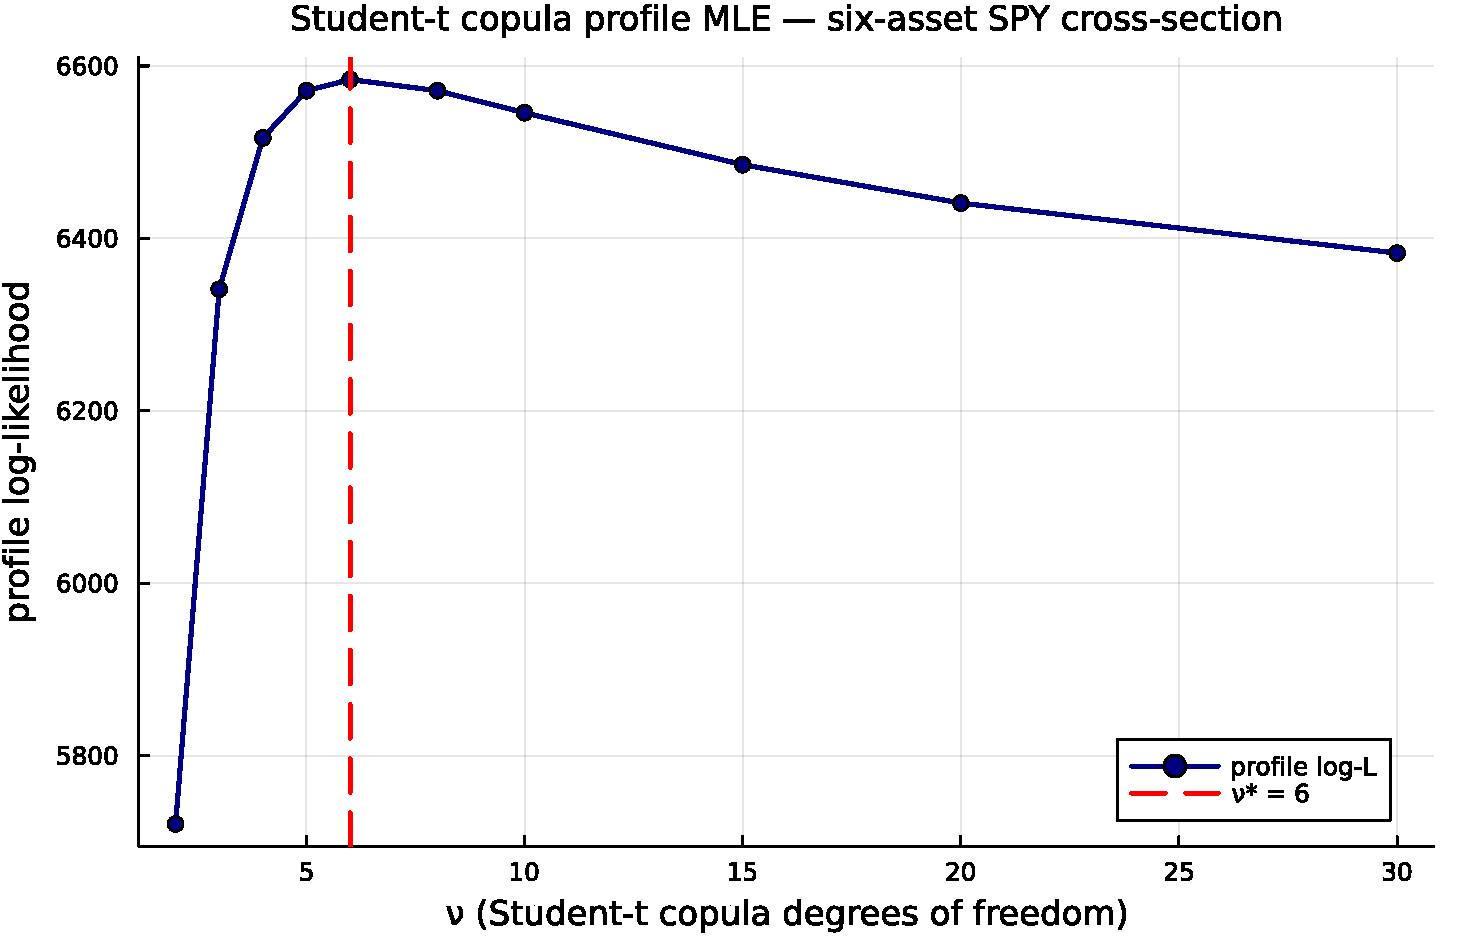
\includegraphics[width=0.70\textwidth]{sections/figs/Fig-v7-Copula-Profile.pdf}
\caption{Profile log-likelihood of the Student-t copula on the six-asset SPY cross-section. The dashed red line marks the profile MLE $\nu^{*} = 6$.}
\label{fig:copula_profile}
\end{figure}

\subsection{Block-Bootstrap Baseline}
\label{sec:block_bootstrap_supp}

Table~\ref{tab:block_bootstrap} reports the full seven-metric panel for the stationary block bootstrap at block length $b = 10$ trading days, the temporally-aware non-parametric baseline added to Table~\ref{tab:model_comparison}.

\begin{table}[h]
\centering
\small
\caption{Stationary block bootstrap (block length $b = 10$ trading days) on SPY (1000 paths, seed = 20260420).}
\label{tab:block_bootstrap}
\begin{tabular}{l cc cc c c c c}
\toprule
Window & KS & AD & Kurt & ACF-MAE & $W_1$ & $H$ & Cov \\
\midrule
IS  & 99.1 & 97.6 & 7.14 & 0.0555 & 0.084 & 0.0504 & 100.0 \\
OoS & 97.7 & 94.6 & 4.03 & 0.0547 & 0.327 & 0.2394 & 100.0 \\
\bottomrule
\end{tabular}
\end{table}

\subsection{Discrete HMM with Bin-Conditional Student-t Emissions}
\label{sec:bin_t_supp}

Table~\ref{tab:bin_t} reports the full seven-metric panel for the Bin-T NJ variant referenced in Section~\ref{sec:model_comparison}: the discrete NJ transition matrix with $K_{\text{disc}} = 13$ quantile bins, but with each bin emitting from a bin-conditional Student-t density rather than from the bin centroid.

\begin{table}[h]
\centering
\small
\caption{Discrete HMM with bin-conditional Student-t emissions on SPY (no jumps, $K_{\text{disc}} = 13$, 1000 paths, seed = 20260420).}
\label{tab:bin_t}
\begin{tabular}{l cc cc c c c c}
\toprule
Window & KS & AD & Kurt & ACF-MAE & $W_1$ & $H$ & Cov \\
\midrule
IS  & 95.5 & 90.3 & 27.28 & 0.0608 & 0.113 & 0.0919 & 84.8 \\
OoS & 97.4 & 96.7 & 5.77  & 0.0587 & 0.298 & 0.2357 & 99.0 \\
\bottomrule
\end{tabular}
\end{table}

The bin-conditional Student-t fit picks $\nu \approx 2.71$ for the two extreme bins (bins $1$ and $13$, corresponding to the lower and upper quantile tails of the IS distribution) and $\nu = 50$ (upper bracket) for the eleven central bins, which explains both the large in-sample simulated kurtosis ($27.28$) and the very thin-scale central bins ($\sigma$ $\sim$ $0.06$--$0.25$).



\subsection{GRU Deep-Generative Baseline}
\label{sec:gru_supp}

Architecture and training details for the GRU baseline used in
Section~\ref{sec:model_comparison} are summarised here.

\begin{itemize}
    \item \textbf{Architecture.} A single-layer Gated Recurrent Unit (GRU)
    with hidden dimension $H = 32$ followed by a Dense head with two
    outputs $(\mu_t, \log \sigma_t)$. Input is a single feature (the
    standardised return) over a context window of $w = 20$ trading days.

    \item \textbf{Loss.} Per-window negative log-likelihood of a Gaussian
    next-step density, equation~\eqref{eq:gru_nll}.

    \item \textbf{Optimiser.} Adam, learning rate $1.0 \times 10^{-3}$.

    \item \textbf{Training schedule.} $20$ epochs, full pass per epoch
    over $T_{\text{IS}} - w$ training windows, randomly shuffled at each
    epoch.

    \item \textbf{Numerical stability.} $\log \sigma_t$ is clamped to
    $[-6, 4]$ inside the loss to prevent gradient explosion when the
    network attempts to assign vanishingly-small variance to extreme
    observations.

    \item \textbf{Pre-processing.} The input return series is standardised
    by its in-sample mean and standard deviation; predictions are
    re-scaled back at sampling time.

    \item \textbf{Synthesis.} The trailing $w$ in-sample returns seed the
    recurrence; for each generation step the predicted Gaussian is
    sampled, the sample is appended to the context window, and the
    procedure rolls forward. The first $64$ steps are discarded as
    burn-in.

    \item \textbf{Implementation.} Julia using \texttt{Flux.jl}
    \cite{innes2018flux} with the \texttt{Optimisers.Adam} state.
    Random seed for weight initialisation, training shuffling, and per-path
    sampling: $V7\_SEED = 20260420$ with deterministic per-path sub-seeds.
\end{itemize}

The trained model is callable through the same
\texttt{simulate\_gru(model, n\_steps; seed\_window)} interface as the
CHMM and discrete-HMM models, so the seven-metric panel evaluates the GRU
on byte-identical windows to the other generators.

\begin{table}[h]
\centering
\small
\caption{GRU deep-generative baseline on SPY (single-layer, hidden $H=32$, window $w=20$, $20$ epochs, Adam $\eta=10^{-3}$, $1{,}000$ paths, seed = 20260420). Final training NLL: $0.2101$.}
\label{tab:gru}
\begin{tabular}{l cc c c c c c}
\toprule
Window & KS & AD & Kurt & ACF-MAE & $W_1$ & $H$ & Cov \\
\midrule
IS  & 2.1  & 2.7  & 2.79 & 0.0526 & 0.174 & 0.0906 & 51.5 \\
OoS & 84.2 & 85.1 & 1.72 & 0.0538 & 0.372 & 0.2441 & 78.8 \\
\bottomrule
\end{tabular}
\end{table}
